    \documentclass[12pt]{article}
\usepackage[scaled]{helvet}
\usepackage[margin=1in]{geometry}
\usepackage[nodisplayskipstretch]{setspace}

\usepackage[utf8]{inputenc}
\usepackage{amsmath}
\usepackage{amsfonts}
\usepackage{multicol, booktabs, bbm, color, xcolor}
\usepackage{natbib}
\usepackage{graphicx}
\usepackage{subcaption}
\usepackage{appendix}
\usepackage{hyperref}
\graphicspath{{./img/}}
\bibliographystyle{apalike}


\begin{document}
\title{Supplemental Material to:\\
``Heterogeneous Distributed Lag Models to Estimate Personalized Effects of Maternal Exposures to Air Pollution''}
\author{Daniel Mork\\ 
Department of Biostatistics\\ Harvard T.H. Chan School of Public Health\\\\

Marianthi-Anna Kioumourtzoglou\\
Department of Environmental Health Sciences\\
Columbia University Mailman School of Public Health\\\\

Marc Weisskopf\\
Department of Environmental Health\\ 
Harvard T.H. Chan School of Public Health\\\\ 

Brent A Coull\\
Department of Biostatistics\\
Harvard T.H. Chan School of Public Health\\\\ 

Ander Wilson\\ 
Department of Statistics\\ Colorado State University}
\date{}

\maketitle
\clearpage
\setstretch{1.3}


%======================================
\section{Model Specification} \label{sec:mod-spec}
%======================================
In the shared tree and Gaussian process HDLMs, the modifier tree specification is identical to the nested tree HDLM. That is, the probability of a split at terminal node $\eta$ with depth $d_\eta$ is $p_{\text{split}}(\eta)=\alpha(1+d_\eta)^{-\beta}$ where $\alpha\in(0,1)$ and $\beta>0$. We set $\alpha=0.95$ and $\beta=2$.

For selecting a splitting rule in the modifier tree, let $\rho=\{m_j,K\}$ define a splitting rule on modifying covariate $m_j$ with splitting set $K$. A splitting set refers to a binary rule that places observations into one of two groups. For continuous $m_j$, $K$ is an inequality and for categorical $m_j$, $K$ is a proper subset of the categories. Define $\psi_j$ to be the probability of selecting modifying covariate $m_j$, $j\in\{1,\ldots,J\}$, to be used for a binary rule. Then, the splitting rule prior is written
\begin{equation}
    p_{\text{rule}}(\rho|\eta)=p(m_j|\eta)p(K|m_j,\eta).
\end{equation}
Here, $p(m_j|\eta)=\psi_j/\sum_j\psi_j\mathbb{I}(m_j\in\mathcal{E}_\eta)$, where $\mathcal{E}_\eta$ is the set of eligible modifiers at node $\eta$. A modifier is eligible if the subgroup at node $\eta$ can be divided into two nonempty subgroups using a binary rule based on that modifier. Also, $p(K|m_j,\eta)$ is the probability of splitting set $K$ for modifier $m_j$ at node $\eta$. For a continuous modifier, $p(K|m_j,\eta)=1\big/(n_{m_j,\eta}-1)$ where $n_{m_j,\eta}$ is the number of splitting locations available for $m_j$ at node $\eta$. If $m_j$ is categorical, $p(K|m_j,\eta)=1\big/(2^{n_{m_j,\eta}-1}-1)$, which is based on the the number of partitions of $n_{m_j,\eta}$ unique values into two non-empty groups. Following \cite{Linero2018}, the prior on probabilities $\boldsymbol\psi=\{\psi_1,\ldots,\psi_J\}$ is
\begin{eqnarray}
    \boldsymbol\psi&\sim&\text{Dirichlet}(\kappa/J,\ldots,\kappa/J)\\
    \frac{\kappa}{\kappa+J}&\sim&\text{Beta}(\zeta,1)
\end{eqnarray}
where $\zeta\in(0.5,1)$. Smaller values of $\zeta$ correspond to increased sparsity of modifiers. We use $\zeta=0.5$ in our simulations and data analysis.

The fixed effects receive a non-informative prior, $\boldsymbol\gamma\sim\mathcal{MVN}(\mathbf{0},c\sigma^2I_p)$ where $c$ is fixed at a large value and $I_p$ is a $p\times p$ identity matrix. The variance parameter $\sigma$ is given a half-Cauchy prior distribution and included in the fixed effects for integration during computation.

\subsection{Tree Priors}
%======================================
\subsubsection{Modifier Tree Priors}
%======================================

The prior on modifier tree structures is defined in two parts: a prior probability that a node will have a split and a prior probability of the binary rule defined at that split. We adopt the BART prior for a node split. That is, for node $\eta$ with depth $d_\eta$ (the first node in a tree has depth zero) the probability the node is an internal node equals $p_{\text{split}}(\eta)=\alpha(1+d_\eta)^{-\beta}$ where $\alpha\in(0,1)$ and $\beta>0$. Following \cite{Chipman2012} we set $\alpha=0.95$ and $\beta=2$, which encourages smaller trees. Changes to these priors did not improve performance in simulations. Priors on tree splitting rules in the modifier tree follow \cite{Linero2018b}.

%======================================
\subsubsection{Treed DLM Priors}
%======================================

The treed DLM uses the BART prior for node splits, with $\alpha=0.95$ and $\beta=2$. For the splitting rule prior, we assign a uniform prior across all available time points, resulting in $T-1$ possible splits for a tree with a single node.



\subsection{Shared Tree HDLM}
Notation for the shared tree HDLM is similar to the nested tree HDLM. For each modifier tree $\mathcal{M}_a$ with terminal nodes $\eta_{ab}$, we consider a single treed DLM $\mathcal{D}_a$ with terminal nodes $\lambda_{ac}$, $c\in\{1,\ldots,C_a\}$. The treed DLM $\mathcal{D}_a$ is utilized as the distributed lag function at all terminal nodes $\eta_{ab}$ of $\mathcal{M}_a$. The distributed lag effects, $\delta_{abc}$, are specific to each modifier tree terminal node and treed DLM terminal node. As in the nested tree DLM, we calculate the heterogeneous DLM by setting $\theta_{abt}=\delta_{abc}$ if $t\in\lambda_{ac}$.


As in the nested tree HDLM, the DLM effects are assigned the conjugate normal prior,
\begin{equation}
    \delta_{abc}|\tau_a,\nu,\sigma\sim\mathcal{N}(0,\tau_a^2\nu^2\sigma^2).
\end{equation}
Variance parameters $\tau_a,\nu,\sigma$ follow a half-Cauchy distribution with scale $=1$ and define a global-local horseshoe-like estimator on tree specific effects. Although the DLM structure and variance is the same for all modifier tree terminal nodes in the shared tree HDLM, each subgroup receives unique distributed lag effect estimates.

\subsection{Gaussian Process HDLM}
We first propose a method for estimating the HDLM using Gaussian processes. Consider a single modifier tree terminal node, $\eta_{ab}$, containing a subset of observations. Let the corresponding $T-$dimensional set of DLM parameters $\boldsymbol\theta_{ab}$ follow a Gaussian process with covariance function $\Sigma_{\boldsymbol\phi}(t,t')$ where $\boldsymbol\phi$ are parameters defining the covariance. We consider the exponential covariance, $\Sigma_{\phi}(t,t')=\exp\{-\phi|t-t'|\}$. An inherent assumption of this approach is that all observations share the same value of $\phi$ due to the computation approach and therefore have the same smoothness over time in their distributed lag functions. Having a common $\phi$ for all nodes on a tree is required due to model computation, which requires integration over the distributed lag function for each subgroup. The equal smoothness assumption may be beneficial if the distributed lag function for all observations have a similar magnitude and window length. In the case where there is a nonzero exposure effect in only a small proportion of the population, the smoothness of the distributed lag function imposed by the remaining sample will make this critical window difficult to estimate. This is because estimation of the smoothing parameter will largely reflect the null group and cause oversmoothing in the group for which there is a non-zero association during some gestational weeks.

We define the Gaussian process prior for the distributed lag function as $\boldsymbol\theta_{ab} |\tau_a,\nu,\sigma,\phi \sim \mathcal{GP}[\mathbf{0},\tau_a^2\nu^2\sigma^2\boldsymbol\Sigma(\phi)]$.
The variance parameters follow a half-Cauchy prior, $\tau_a,\nu\sim\mathcal{C}^+(0,1)$, to define a local-global horseshoe-like estimator on tree specific effects \citep{Carvalho2010}. This differs from previous BART implementations \citep{Chipman2012,Starling2019}, which apply a uniform variance across all trees. The horseshoe variance prior will shrink the effects of misspecified trees reducing variance and false window detection. A similar prior specification was shown to improve DLM estimation in the treed DLM method of \cite{Mork2023EstimatingPairs}. We restrict the range of $\phi$ to $\exp\{-\phi\}\in(0.05, 0.95)$ and assign prior $\phi\sim\text{Gamma}(1/2,1/2)$ truncated over the range of $\phi$, which gives higher probability to a smoother distributed lag function.

The Gaussian process prior for DLM effects is
\begin{equation}
    \boldsymbol\theta_{ab}|\tau_a,\nu,\sigma,\phi\sim\mathcal{GP}[\mathbf{0},\tau_a^2\nu^2\sigma^2\Sigma(\phi)].
\end{equation}
Variance parameters $\tau_a,\nu,\sigma$ follow a half-Cauchy distribution with scale $=1$ and define a global-local horseshoe-like estimator on tree specific effects. We use the exponential covariance matrix $\Sigma(\phi)$ with range parameter $\phi$ and restrict the range such that $\exp\{-\phi\}\in(0.05,0.95)$. That is, the lag-1 covariance is between 0.05 and 0.95. We assign prior $\phi\sim\text{Gamma}(1/2,1/2)$, which gives higher probability to more smoothness in the HDLM.




%======================================
\section{Computational Approach} 
%======================================
We describe the computation approach of the treed HDLMs in general and note where the algorithm changes depending on the method. The algorithm is based on the approach described by \citep{Chipman2012} with differences to accommodate fixed effects, multivariate predictors, and the treed DLM for estimation of a vector of structured regression coefficients.

\subsection{Preprocessing}
Before running the treed HDLM algorithm, we perform the following operations to promote computational precision and mitigate numerical overflow issues:
\begin{itemize}
    \item The response, $\mathbf{y}$, is centered to have mean zero and scaled to have a range equal to 1.
    \item Continuous covariates are centered to have mean zero and all covariates are scaled by their $\ell_2$ norm such that $\mathbf{Z}^T\mathbf{Z}$ has a diagonal of ones.
    \item Exposure data is scaled to have standard deviation 1.
\end{itemize}


\subsection{Modifier tree update}
\subsubsection{Marginalizing out fixed effect parameters}
Consider the distribution of the data $\mathbf{y}_i\sim\mathcal{N}[f(\mathbf{x_i},\mathbf{m}_i)+\mathbf{z}^T\boldsymbol\gamma,\sigma^2]$, where $f(\mathbf{x_i},\mathbf{m}_i)=\boldsymbol\theta(\mathbf{m}_i)$ is the heterogeneous distributed lag effects for individual $i$. The posterior distribution of $\boldsymbol\gamma$ is
\begin{equation}
    p(\boldsymbol\gamma|\mathbf{y},\mathbf{f},\sigma^2)\propto
    \sigma^{-p/2}|\mathbf{V}_{\boldsymbol\gamma}|^{-1/2}
    \exp\left\{-\sigma^{-2}(\mathbf{y}-\mathbf{f})^T\mathbf{Z}^T\mathbf{V}_{\boldsymbol\gamma}^{-1}\mathbf{Z}(\mathbf{y}-\mathbf{f})\right\}.
\end{equation}
Here, $\mathbf{y}=[y_1,\ldots,y_n]^T$ is a vector of our continuous response; $\mathbf{f}=[f(\mathbf{x}_1,\mathbf{m}_1),\ldots,f(\mathbf{x}_n,\mathbf{m}_n)]'$ where $\mathbf{Z}$ is a matrix of covariates such that row $i$ equals $\mathbf{z}_i^T$. In addition,
\begin{equation}\label{eq:Vgamma}
    \mathbf{V}_{\boldsymbol{\gamma}}=(\mathbf{Z}^T\mathbf{Z}+\mathbf{I}/c)^{-1},
\end{equation}
where $c$ is a fixed at a large value indicating a non-informative prior on $\boldsymbol\gamma$.

In the treed HDLMs, the heterogeneous distributed lag function $f(\mathbf{x}_i,\mathbf{m}_i)$ is estimated by the sum of partial distributed lag functions. In order to account for the effect of covariates $\mathbf{z}_i$ when estimating the trees, we integrate over the parameters $\boldsymbol\gamma$. This results in the marginal distribution for our data,
\begin{equation}
    \mathbf{y}|\mathbf{f},\sigma^2\sim\mathcal{MVN}(\mathbf{f},\sigma^2\mathbf{V}_{\mathbf{Z}}),
\end{equation}
where
\begin{equation}
    \mathbf{V}_{\mathbf{Z}}=(\mathbf{I}-\mathbf{Z}\mathbf{V}_{\boldsymbol\gamma}\mathbf{Z}^T)^{-1}.
\end{equation}

\subsubsection{Bayesian backfitting}
The update of each modifier tree, $a=1,\ldots,A$, proceeds using Bayesian backfitting \citep{Hastie2000}. First, we calculate $\mathbf{R}_a$, the partial residuals after removing the effects of all other trees. We define $\mathbf{R}_a$ as
\begin{equation}\label{eq:dlm-resid}
    \mathbf{R}_{a}=\mathbf{y}-\sum_{\substack{a'=1\\a'\not=a}}^A g(\mathbf{X}, \mathcal{T}_{a'}).
\end{equation}
Here, $g(\mathbf{X}, \mathcal{T}_{a})$ is the vector of partial distributed lag estimates due to modifier tree $\mathcal{T}_{a}$ and corresponding distributed lag effects for each modifier tree terminal node. In the case of nested tree HDLM, $\mathcal{T}_{a}$ encompasses the nested treed DLMs: $\mathcal{D}_{a1},\ldots,\mathcal{D}_{aB_a}$. In the case of shared tree HDLM, $\mathcal{T}_a$ includes the shared treed DLM $\mathcal{D}_a$.

Let $\mathbb{X}_a=[\mathbf{X}_{a1},\ldots,\mathbf{X}_{aB_a}]$ denote a block-style exposure data matrix for modifier tree $a$. Each $\mathbf{X}_{ab}$ is a $n\times T$ matrix that corresponds to the exposure data for modifier terminal node $\eta_{ab}$. The non-zero rows of $\mathbf{X}_{ab}$ are exposure observations for the subgroup defined by the rules leading to $\eta_{ab}$; other rows are equal to zero.

The distribution of the partial distributed lag effects is
\begin{equation}
    \label{eq:Ra-partial-dlnm-dist}
    \mathbf{R}_a|- \sim \mathcal{MVN}\left(\mathbb{X}_a\Theta_{a},\sigma^2\mathbf{V_Z} \right)
\end{equation}
where $\Theta_a=[\boldsymbol\theta_{a1}',\ldots,\boldsymbol\theta_{aB_a}']'$ represents a vector of distributed lag parameters parameters corresponding to the subgroups of modifier tree $\mathcal{T}_a$. In the case of nested and shared tree HDLMs, sets of the $\boldsymbol\theta_{ab}$ parameters are equal based on the piecewise constant structure of the treed DLM \citep{Mork2023EstimatingPairs}.
    
\subsubsection{Tree prosposal}
We update each $\mathcal{T}_{a}$, using a Metropolis-Hastings algorithm. We consider a proposal distribution with transition steps as follows:
\begin{itemize}
    \item Grow: Randomly select a terminal node, $\eta$, to grow. Randomly select a splitting rule according to $p_{\text{rule}}(\rho|\eta)$ and create two new terminal nodes using the new splitting rule along with all previous rules.
    \item Prune: Randomly select an internal node with exactly two terminal nodes descending from it and remove the splitting rule.
    \item Change: Randomly select any internal node, $\eta$, and define a new splitting rule according to $p_{\text{rule}}(\rho|\eta)$. Update the limits of all terminal nodes that branch from $\eta$.
    \item Swap: Randomly select two connected internal nodes and reverse the rule ordering. That is, the parent node splitting rule and the child node splitting rule trade places.
\end{itemize}

The grow and prune steps are counterparts to one another, while change and swap are their own counterparts that can reverse the Markov chain. The transition kernel $p(\mathcal{T}^*|\mathcal{T})$ is given by the probability of selecting a step, multiplied by the probabilities associated with that step. For our simulations and data analysis we draw a new proposal from the four options (grow, prime, change, swap). The probability of using a grow or prune proposal is 0.25, change is 0.4, and swap 0.1.

\subsubsection{Nested tree proposal}
In the nested tree HDLM, a grow and prune proposal also requires new nested treed DLMs. In particular, a modifier tree grow proposal creates two new terminal nodes, requiring a new treed DLM at each node. A prune proposal removes two previous terminal nodes and requires a new treed DLM at the resulting pruned node.

A nested treed DLM is drawn from the tree prior using a stochastic growing process. At each terminal node, $\lambda_c$ of the treed DLM, a split occurs with probability $p_{\text{split}}(\lambda_c)=\alpha(1+d_\lambda)^{-\beta}$ (see Section \ref{sec:mod-spec} of Supplemental Material). If a split occurs, a time-point split in the DLM is selected with uniform probability over the remaining time points. This process repeats until no splits occur or there are no remaining time points. The hyperparameters $\alpha$ and $\beta$ encourage small trees, which is necessary to retain constraints on the distributed lag effects. 

\subsubsection{Accepting a modifier tree proposal}\label{sec:accept-mod-tree}
After a new modifier tree proposal is made, we accept it by a standard Metropolis-Hastings ratio. To eliminate the need for complicated procedures due to the change in parameter dimension and to make the trees invariant to the covariates and variance, we integrate over $\Theta_a$ as well as $\sigma^2$. In BART, integrating out the vector $\Theta_a$ can be done one parameter at a time, as each observation is restricted to a single terminal node. However, in the treed HDLMs, the resulting covariance after integrating out fixed effect parameters $\boldsymbol\gamma$, requires us to simultaneously integrate over all distributed lag parameters for modifier tree $\mathcal{T}_a$. The marginal likelihood of $\mathbf{R}_a$ is calculated to be
\begin{equation}
\begin{split}
p(\mathbf{R}_a|\mathcal{T}_{a_j}-) &=
\int_{\sigma^2}\int_{\Theta_a}
 p(\mathbf{R}_{a}|\Theta_a,\mathcal{T}_{a},-) 
 p(\Theta_a|\mathcal{T}_a,-) 
 p(\sigma^2)\; 
 d\Theta_a\; d\sigma^2\\
&=\left(\nu^2\tau_a^2\right)^{-P_a/2}\\
&\phantom{=}
\times\left\vert\mathbf{V}_{\Theta_a}\right\vert^{1/2}
\left[\frac{\mathbf{R}_a^T\left(\mathbf{I}_n-
    \mathbf{Z}^T\mathbf{V}_{\boldsymbol{\gamma}}\mathbf{Z}-
    \mathbf{V}_\mathbf{Z}^{-1}\mathbb{X}_a \mathbf{V}_{\Theta_a} \mathbb{X}_a^T \mathbf{V}_\mathbf{Z}^{-1}\right)
\mathbf{R}_a}{2}+\frac{1}{\xi_{\sigma^2}}\right]^{-(n+1)/2}
\end{split}
\end{equation}
where $\xi_{\sigma^2}$ is from the hierarchy  $\sigma^2|\xi_{\sigma^2}\sim\mathcal{IG}(1/2,1/\xi_{\sigma^2})$ and $\xi_{\sigma^2}\sim\mathcal{IG}(1/2,1)$, which results in $\sigma\sim\mathcal{C}^+(0,1)$; and $P_a$ is the number of unique parameters in $\Theta_a$ (for the Gaussian process HDLM, $P_a=TB_a$, for the shared tree HDLM, $P_a=C_aB_a$, and for the nested tree HDLM, $P_a=\sum_{b=1}^{B_a}C_{ab}$). Finally,
\begin{equation}
    \mathbf{V}_{\Theta_a}=\left(\mathbb{X}_a^T \mathbf{V}_\mathbf{Z}^{-1}\mathbb{X}_a+\nu^{-2}\tau_a^{-2}\mathbf{U}_a\right)^{-1},
\end{equation}
where $\mathbf{U}_a$ is a diagonal block matrix of $\Sigma(\phi)$ for the Gaussian process HDLM, or an identity matrix for the shared and nested HDLMs. We note that use of the Woodbury matrix identity gives a more efficient method of calculating $\mathbf{V}_{\Theta_a}$.

After integrating over tree-specific parameters, we calculate $p(\mathbf{R}_a,\mathcal{T}_{a}|-)=p(\mathbf{R}_a|\mathcal{T}_{a},-)p(\mathcal{T}_{a})$ and accept $\mathcal{T}_{a}^*$ according to the Metropolis-Hastings ratio given by
\begin{equation}\label{eq:single_mh}
r=\min\left\{1,\frac{p(\mathcal{T}_{a}^*)p(\mathbf{R}_a|\mathcal{T}_{a}^*,-)p(\mathcal{T}_{a}\vert\mathcal{T}_{a}^*)}{p(\mathcal{T}_{a})p(\mathbf{R}_a|\mathcal{T}_{a},-)p(\mathcal{T}_{a}^*\vert \mathcal{T}_{a})}\right\}.
\end{equation}



\subsection{Treed DLM update}
For the shared tree HDLM, a single treed DLM, $\mathcal{D}_a$, is updated for every modifier tree, $\mathcal{T}_a$. In the nested tree HDLM, a nested treed DLM, $\mathcal{D}_{ab}$ is updated for each modifier tree terminal node $\eta_{ab}$. Proposals for the treed DLMs occur through grow, prune, and change steps, and use a uniform prior over the remaining time splitting points. See \cite{Mork2023EstimatingPairs} for more details.

After a new treed DLM has been proposed, it is accepted with the independent Metropolis-Hastings algorithm. This process is identical to that described for modifier trees in Section \ref{sec:accept-mod-tree}.



\subsection{Full conditionals}
After each modifier tree update (and treed DLM updates for shared and nested HDLMs), we draw $\Theta_a$ (all parameters specific to modifier tree $a$) from the full conditional distribution,
\begin{equation}\label{eq:mu-posterior}
    \Theta_a|-\sim \mathcal{MVN}_{P_a}\left(\mathbf{V}_{\Theta_a}\mathbb{X}_a^T \mathbf{V}_\mathbf{Z}^{-1}\mathbf{R}_a,\sigma^2 \mathbf{V}_{\Theta_a}\right).
\end{equation}

The update of trees and corresponding partial HDLM is followed by a draw from the full conditional of remaining parameters and hyperparameters:
\begin{equation}
    \xi_{\sigma}|- \sim \mathcal{IG}\left(1,1+\frac{1}{\sigma^2}\right);
\end{equation}
\begin{equation}
    \sigma^2|- \sim \mathcal{IG}\left[\frac{n+P+1}{2}, 
    \frac{\Vert \mathbf{V}_{\mathbf{Z}}^{-1/2} (\mathbf{y}-\mathbf{f}) \Vert_2^2}{2} +\frac{D}{2\nu^2}+\frac{1}{\xi_{\sigma}}\right];
\end{equation}
where $P=\sum_{a=1}^A P_a$ and $D=\sum_{a=1}^A \Theta_a^T\mathbf{U}_a\Theta_a/\tau_a^2$. Also,
\begin{equation}
    \xi_{\nu}|- \sim \mathcal{IG}\left(1,1+\frac{1}{\nu^2}\right);
\end{equation}
\begin{equation}
    \nu^2|- \sim \mathcal{IG}\left(\frac{P+1}{2},
    \frac{D}{2\sigma^2} + \frac{1}{\xi_{\nu}}\right);
\end{equation}
\begin{equation}
    \xi_{\tau_{a}}|- \sim \mathcal{IG}\left(1,1+\frac{1}{\tau_{a}^2}\right);
\end{equation}
\begin{equation}
    \tau_a^2|- \sim \mathcal{IG}\left(\frac{P_a+1}{2}, \frac{\Theta_a^TU_a\Theta_a}{2\sigma^2\nu^2} + \frac{1}{\xi_{\tau_a}}\right).
\end{equation}

Updates of modifier selection probabilities $\boldsymbol\psi$ come from full conditional
\begin{equation}
    \boldsymbol\psi|-\sim\text{Dirichlet}\left(\kappa/J+N_{\{m_j=1\}},\ldots,\kappa/J+N_{\{m_j=M\}}\right)
\end{equation}
where $N_{\{m_j=m\}}$ is the number of splitting rules using modifier $m$. The hyperprior $\kappa$ is updated by the Metropolis-Hastings algorithm.

Finally we draw $\boldsymbol{\gamma}$ from its full conditional,
\begin{equation}
    \boldsymbol{\gamma}|\mathbf{y},\mathbf{f},\sigma^2 \sim \mathcal{MVN}\left[\mathbf{V}_{\boldsymbol{\gamma}}\mathbf{Z}(\mathbf{y}-\mathbf{f}), \sigma^2 \mathbf{V}_{\boldsymbol{\gamma}}\right].
\end{equation}

\subsection{Subgroup posterior analysis}
The HDLM framework allows for inference on personalized distributed lag functions for a specific level of modifiers or subgroup specific distributed lag estimates averaged over the levels of modifiers within a particular subgroup. Let $S$ be a set of observations based on a subgroup of interest. For example, S may be the set of all babies born to Hispanic mothers or all boy babies with obese mothers. Denote $S_{\eta_{ab}}\subset S$ as the observations from $S$ contained in modifier tree terminal node $\eta_{ab}$. Then, we define weights based on the proportion of $S$ in each terminal node, $w(S,\eta_{ab})=|S_{\eta_{ab}}|\big/|S|$. The DLM for subgroup $S$ is calculated
\begin{equation}
    \boldsymbol\theta_S=\sum_{a=1}^A\sum_{b=1}^{B_a}\boldsymbol\theta_{ab}w(S,\eta_{ab})
\end{equation}
where $\boldsymbol\theta_{ab}$ is the vector of DLM effects for modifier tree terminal node $\eta_{ab}$.


%======================================
\section{Additional Simulation Results} 
%======================================
Code and descriptions to replicate simulation results are available at \url{https://github.com/danielmork/HDLM}.
\subsection{Scenario 1: Early/Late Window}
Table \ref{tab:scen1_res} presents simulation results from Scenario 1 including Gaussian process HDLM and DLM.

\begin{table}[!ht]
\scriptsize
    \centering
    \caption{Simulation results for estimating the DLM in scenario 1 (early/late effect). Results are considered pointwise across the DLM for each individual and broken down for individuals with a zero versus nonzero effect. }\vspace{6pt}
    \label{tab:scen1_res}
    \begin{tabular}{lrrrrrrrr}
        \toprule[2pt]
        &\multicolumn{4}{c}{Effect ($z_{i1}>0$)}&&\multicolumn{3}{c}{No Effect ($z_{i1}\leq0$)}\\
        \cmidrule(lr){2-5} \cmidrule(lr){7-9} 
        Model & RMSE$^*$ & Coverage & TP & FP & \phantom{} &RMSE$^*$ & Coverage & FP\\
        \midrule
        \multicolumn{9}{l}{$\sigma^2=1$}\\
      Nested Tree HDLM & 1.94 & 0.97 & 1.00 & 0.02 &  & 1.88 & 0.99 & 0.01 \\
      Shared Tree HDLM & 2.15 & 0.97 & 0.99 & 0.02 &  & 1.97 & 0.97 & 0.03 \\
 Gaussian Process HDLM & 3.24 & 0.95 & 0.99 & 0.03 &  & 2.46 & 0.98 & 0.02 \\
\addlinespace
            Treed DLM & 10.87 & 0.61 & 1.00 & 0.22 &  & 5.71 & 0.61 & 0.39\\
               Gaussian Process DLM & 10.97 & 0.61 & 1.00 & 0.23 &  & 5.67 & 0.61 & 0.39 \\
\addlinespace
   Nested Tree: Truth & 0.74 & 0.99 & 1.00 & 0.01 &  & 0.47 & 1.00 & 0.00   \\
     Gaussian Process: Truth & 2.76 & 0.96 & 1.00 & 0.03 &  & 1.77 & 0.98 & 0.02   \\


\midrule
        
        \multicolumn{9}{l}{$\sigma^2=25$}\\
        Nested Tree HDLM & 6.29 & 0.92 & 0.90 & 0.04 &  & 2.67 & 1.00 & 0.00 \\
        Shared Tree HDLM & 7.03 & 0.91 & 0.88 & 0.05 &  & 3.25 & 0.99 & 0.01 \\
   Gaussian Process HDLM & 6.99 & 0.95 & 0.92 & 0.02 &  & 4.02 & 1.00 & 0.00 \\
\addlinespace
              Treed DLM & 11.49 & 0.65 & 0.81 & 0.17 &  & 5.42 & 0.69 & 0.31 \\
   Gaussian Process DLM & 11.52 & 0.70 & 0.63 & 0.11 &  & 5.47 & 0.78 & 0.22 \\
\addlinespace
      Nested Tree: Truth & 5.26 & 0.96 & 0.95 & 0.02 &  & 2.10 & 1.00 & 0.00  \\
 Gaussian Process: Truth & 6.37 & 0.96 & 0.98 & 0.02 &  & 3.71 & 1.00 & 0.00  \\
        \bottomrule[2pt]
        \multicolumn{9}{l}{*RMSE$\times100$}\\
    \end{tabular}
\end{table}

Table \ref{tab:scen1_inc} presents modifier posterior inclusion probabilities for Scenario 1.

\begin{table}[!ht]
 \footnotesize
    \centering
    \caption{Simulation results for modifier inclusion in scenario 1 (early/late effect). Results describe the average posterior inclusion probability across simulation replicates for each potential modifier, ($z_i$) or group of modifiers ($z_{[i-j]}$) in any tree of the model. A value of one indicates the modifier was always present in at least one tree of the model.}
    \label{tab:scen1_inc}
    \begin{tabular}{lrrrrr}
        \toprule[2pt]
        Model & $z_{1}^*$ & $z_{2}^*$ & $z_{3}$ & $z_{[4-8]}$ & $z_{[9-13]}$ \\
        
        
        \midrule
        \multicolumn{6}{l}{$\sigma^2=1$}\\
Nested Tree HDLM & 1.00 & 1.00 & 0.54 & 0.55 & 0.52\\
Shared Tree HDLM & 1.00 & 1.00 & 0.55 & 0.55 & 0.51\\
Gaussian Process HDLM & 1.00 & 1.00 & 0.58 & 0.59 & 0.56\\
    
        \midrule
        \multicolumn{6}{l}{$\sigma^2=25$}\\
Nested Tree HDLM & 1.00 & 0.97 & 0.62 & 0.62 & 0.60\\
Shared Tree HDLM & 1.00 & 0.97 & 0.62 & 0.62 & 0.60\\
Gaussian Process HDLM & 1.00 & 0.99 & 0.62 & 0.62 & 0.60\\

        \bottomrule[2pt]
        \multicolumn{6}{l}{$^*$ active modifiers in scenario 1}\\
    \end{tabular}
\end{table}



Table \ref{tab:scen1_inc2} presents modifier interaction posterior inclusion probabilities (PIP). An modifier interaction occurs when two modifiers are used in consecutive splitting rules in the same tree. For simulation scenario 1, we would expect modifiers $z_1$ and $z_2$ to be used in consecutive splitting rules due to how the distributed lag effects are defined. We see in the lowest error setting the modifier interaction PIP for $z_{1/2}$ (interaction between modifiers $z_1$ and $z_2$) is 1 for all HDLMs. In the medium error scenario this decreases slightly to a PIP of 0.88 for the nested tree HDLM; for the highest error scenario this is 0.46. 

\begin{table}[!ht]
\footnotesize
    \centering
    \caption{Simulation results for modifier interaction posterior inclusion probabilities (PIP) in scenario 1 (early/late effect). Interaction PIP indicates the probability a pair of modifiers was used for two consecutive splitting rules in the same tree at least once in the ensemble. We report the average across simulation replicates of the correct interaction PIP, $z_{1/2}$, the average PIP of other interactions, $z_{i/j}$ and the maximum PIP of other interactions, $\max z_{i/j}$.}\vspace{6pt}
    \label{tab:scen1_inc2}
    \begin{tabular}{lrrr}
        \toprule[2pt]
        Model & $z_{1/2}$ & $z_{i/j}$ & $\max z_{i/j}$\\
        \midrule
        \multicolumn{4}{l}{$\sigma^2=1$}\\
Nested Tree HDLM & 1.00 & 0.10 & 0.55\\
Shared Tree HDLM & 1.00 & 0.10 & 0.74\\
Gaussian Process HDLM & 1.00 & 0.11 & 0.57\\

        \midrule
        \multicolumn{4}{l}{$\sigma^2=25$}\\
Nested Tree HDLM & 0.88 & 0.12 & 0.40\\
Shared Tree HDLM & 0.89 & 0.12 & 0.42\\
Gaussian Process HDLM & 0.93 & 0.12 & 0.41\\

        \bottomrule[2pt]
    \end{tabular}
\end{table}


We also tracked the average PIP of other modifier interactions as well as the maximum PIP of other modifier interactions. The average was around 0.12 while the maximum PIP of modifier interactions ranged from 0.40 to 0.44. These results give a relative measure for modifier interaction importance in our data analysis. That is, modifier interactions larger than 0.44 may represent meaningful differences in the distributed lag effects.


\subsection{Scenario 2: Scaled Effect}
Table \ref{tab:scen2_res} presents simulation results from scenario 2 including Gaussian process HDLM and DLM.

\begin{table}[!ht]
 \scriptsize
    \centering
    \caption{Simulation results for estimating the DLM in scenario 2 (scaled effect). Results are considered pointwise across the DLM for each individual and broken down for individuals with a zero versus nonzero effect.}\vspace{6pt}
    \label{tab:scen2_res}
    \begin{tabular}{lrrrrrrrrr}
        \toprule[2pt]
        &\multicolumn{4}{c}{Effect ($z_{i1}>0$)}&&\multicolumn{3}{c}{No Effect ($z_{i1}\leq0$)}\\
        \cmidrule(lr){2-5} \cmidrule(lr){7-9} 
        Model & RMSE$^*$ & Coverage & TP & FP & \phantom{a} &RMSE$^*$ & Coverage & FP \\
        \midrule
        \multicolumn{9}{l}{$\sigma^2=1$}\\
      Nested Tree HDLM & 2.73 & 0.91 & 0.93 & 0.02 &  & 1.73 & 0.99 & 0.01\\
      Shared Tree HDLM & 2.50 & 0.92 & 0.95 & 0.02 &  & 1.77 & 0.98 & 0.02 \\
 Gaussian Process HDLM & 3.73 & 0.95 & 0.86 & 0.02 &  & 2.40 & 0.99 & 0.01 \\
\addlinespace
             Treed DLM & 9.84 & 0.79 & 1.00 & 0.01 &  & 6.39 & 0.78 & 0.22 \\
               Gaussian Process DLM & 10.13 & 0.79 & 1.00 & 0.02 &  & 6.25 & 0.76 & 0.24 \\
\addlinespace
MSPE Selected Model & 2.52 & 0.92 & 0.94 & 0.02 &  & 1.73 & 0.99 & 0.01  \\
WAIC Selected Model & 2.62 & 0.91 & 0.95 & 0.02 &  & 1.75 & 0.99 & 0.01   \\
        \midrule
        
        
        \multicolumn{9}{l}{$\sigma^2=25$}\\
              Nested Tree HDLM & 6.43 & 0.92 & 0.66 & 0.01 &  & 2.60 & 1.00 & 0.00 \\
      Shared Tree HDLM & 6.23 & 0.93 & 0.73 & 0.01 &  & 2.85 & 0.99 & 0.01\\
 Gaussian Process HDLM & 7.43 & 0.94 & 0.64 & 0.01 &  & 3.90 & 1.00 & 0.00 \\
\addlinespace
            Treed DLM & 10.83 & 0.82 & 0.92 & 0.02 &  & 5.81 & 0.79 & 0.21 \\
               Gaussian Process DLM & 11.06 & 0.84 & 0.89 & 0.01 &  & 5.76 & 0.80 & 0.20 \\
\addlinespace
MSPE Selected Model & 6.05 & 0.93 & 0.70 & 0.01 &  & 2.74 & 1.00 & 0.00   \\
WAIC Selected Model & 6.32 & 0.92 & 0.72 & 0.01 &  & 2.75 & 0.99 & 0.01   \\
        
        
        \bottomrule[2pt]
        \multicolumn{9}{l}{*RMSE$\times100$}\\
    \end{tabular}
\end{table}

Table \ref{tab:scen2_inca} presents posterior inclusion probabilities for an individual modifier.

\begin{table}[!ht]
 \scriptsize
    \centering
    \caption{Simulation results for modifier inclusion in scenario 2 (scaled effect). Results describe the average posterior inclusion probability across simulation replicates for each potential modifier (or group of modifiers) in any tree of the model. A value of one indicates the modifier was always present in at least one tree of the model.}\vspace{6pt}
    \label{tab:scen2_inca}
    \begin{tabular}{lrrrrr}
        \toprule[2pt]
        Model & $z_1^*$ & $z_2$ & $z_3^*$ & $z_{[4-8]}$ & $z_{[9-13]}$\\
        
        \midrule
        \multicolumn{6}{l}{$\sigma^2=1$}\\
Nested Tree HDLM & 1.00 & 0.44 & 1.00 & 0.49 & 0.45\\
Shared Tree HDLM & 1.00 & 0.49 & 1.00 & 0.52 & 0.49\\
Gaussian Process HDLM & 1.00 & 0.42 & 1.00 & 0.48 & 0.43\\
       
        \midrule
        \multicolumn{6}{l}{$\sigma^2=25$}\\
Nested Tree HDLM & 1.00 & 0.59 & 0.98 & 0.61 & 0.59\\
Shared Tree HDLM & 1.00 & 0.59 & 0.98 & 0.62 & 0.59\\
Gaussian Process HDLM & 1.00 & 0.58 & 0.98 & 0.61 & 0.59\\
        \bottomrule[2pt]
        \multicolumn{6}{l}{$^*$ active modifiers in scenario 2}\\
    \end{tabular}
\end{table}

Table \ref{tab:scen2_inc} presents modifier interaction PIPs for simulation scenario 2. Here, we show the PIP of the active interactions, $z_{1/3}$ and $z_{3/3}$. Because scenario 2 had a continuous effect, it is reasonable that the tree may split on the modifier $z_3$ multiple times. However, other trees in the ensemble that split on $z_1$ may split on $z_3$ at a different location to build the scaled distributed lag effect.
\begin{table}[!ht]
\footnotesize
    \centering
    \caption{Simulation results for modifier interaction posterior inclusion probabilities (PIP) in scenario 2 (scaled effect). Interaction PIP indicates the probability a pair of modifiers was used for two consecutive splitting rules in the same tree at least once in the ensemble. We report the average across simulation replicates of the correct interaction PIPs, $z_{1/3}$ and $z_{3/3}$, the average PIP of other interactions, $z_{i/j}$ and the maximum PIP of other interactions, $\max z_{i/j}$.}\vspace{6pt}
    \label{tab:scen2_inc}
    \begin{tabular}{lrrrr}
        \toprule[2pt]
        Model & $z_{1/3}$ & $z_{3/3}$ & $z_{i/j}$ & $\max z_{i/j}$\\
        \midrule
        \multicolumn{5}{l}{$\sigma^2=1$}\\
Nested Tree HDLM & 1.00 & 0.86 & 0.08 & 0.55\\
Shared Tree HDLM & 1.00 & 1.00 & 0.09 & 0.49\\
Gaussian Process HDLM & 1.00 & 0.87 & 0.08 & 0.54\\
        
       
        \midrule
        \multicolumn{5}{l}{$\sigma^2=25$}\\
Nested Tree HDLM & 0.91 & 0.34 & 0.11 & 0.35\\
Shared Tree HDLM & 0.94 & 0.36 & 0.11 & 0.38\\
Gaussian Process HDLM & 0.91 & 0.37 & 0.11 & 0.41\\

        \bottomrule[2pt]
    \end{tabular}
\end{table}

We find that the modifier interaction PIP for $z_{1/3}$ is 1 in the lowest error scenario, 0.91 in the middle error case, and 0.65 in the largest error setting. The $z_{3/3}$ modifier is larger than other modifiers on average, but does not always exceed the maximum value of other modifiers. Here, we see average and maximum PIPs for other modifiers similar to results in scenario 1.



%======================================
\subsection{Scenario 3: No Effect Heterogeneity}
%======================================
In the final simulation scenario we considered a DLM without effect modification. The distributed lag effects were defined $\theta_t(\mathbf{m}_i)=\max[0,(t-s)(s-t+9)]$, where $s$ is a starting time drawn uniformly from $\{1,\ldots,T-9\}$. That is, the distributed lag function is smooth with a critical window over an 8-week time period. The distributed lag function is identical for all observations in a given dataset.

Table \ref{tab:scen3_res} presents results for estimation of the distributed lag function. The HDLM performed on par with standard DLM methods without heterogeneity. The HDLM methods had higher RMSE than standard treed DLM and were similar to the Gaussian process DLM. Coverage of the true distributed lag function by 95\% pointwise credible intervals met the nominal level. The TP rates from the HDLM methods were slightly below those from the DLM methods without effect heterogeneity while the FP rate was near zero for all methods. The tree-based HDLMs outperformed the Gaussian process DLM in the higher noise setting; these results encourage the use of tree-based approaches for estimating a DLM or HDLM in general. We also noticed that both non-heterogeneous DLMs and HDLMs were sometimes selected by MSPE, although results for the MSPE selected model were similar to results from standard treed DLM.

\begin{table}[!ht]
 \scriptsize
    \centering
    \caption{Simulation results for estimating the DLM in scenario 3 (no effect heterogeneity). Results are considered pointwise across the DLM for each individual. Selected indicates the proportion of replicates for which a given method had lowest MSPE, calculated using 5,000 out of sample observations.}\vspace{6pt}
    \label{tab:scen3_res}
    \begin{tabular}{lrrrrr}
        \toprule[2pt]
        Model & RMSE$\times100$ & Coverage & TP & FP & Selected\\
        \midrule
        \multicolumn{6}{l}{$\sigma^2=1$}\\
Nested Tree HDLM & 1.18 & 0.95 & 1.00 & 0.00 & 0.24\\
Shared Tree HDLM & 1.18 & 0.95 & 1.00 & 0.00 & 0.20\\
Gaussian Process HDLM & 1.35 & 0.98 & 1.00 & 0.02 & 0.04\\
\addlinespace
Treed DLM & 0.95 & 0.98 & 1.00 & 0.01 & 0.52\\
Gaussian Process DLM & 1.33 & 0.97 & 1.00 & 0.03 & 0.00\\
\addlinespace
MSPE Selected & 0.98 & 0.97 & 1.00 & 0.01 & \\
\midrule

        \multicolumn{6}{l}{$\sigma^2=25$}\\
Nested Tree HDLM & 3.42 & 0.97 & 0.76 & 0.00 & 0.22\\
Shared Tree HDLM & 3.35 & 0.97 & 0.76 & 0.00 & 0.27\\
Gaussian Process HDLM & 3.84 & 1.00 & 0.76 & 0.00 & 0.08\\
\addlinespace
Treed DLM & 3.01 & 0.98 & 0.82 & 0.01 & 0.38\\
Gaussian Process DLM & 3.64 & 0.99 & 0.89 & 0.01 & 0.05\\
\addlinespace
MSPE Selected & 3.11 & 0.98 & 0.80 & 0.00 & \\
        \bottomrule[2pt]
    \end{tabular}
\end{table}



Table \ref{tab:scen3_inc} presents modifier interaction PIPs for simulation scenario 3 (no effect heterogeneity). In this scenario, no modifier interaction plays a role in modeling the distributed lag effect. We find that the average PIP for modifier interactions is 0.12 and the maximum PIP ranges from 0.24 to 0.27 across all error settings. The fact that no one modifier interaction stands out bodes well for the model estimating distributed lag effects without heterogeneity.

\begin{table}[!ht]
\footnotesize
    \centering
    \caption{Simulation results for modifier interaction posterior inclusion probabilities (PIP) in scenario 3 (no effect heterogeneity). Interaction PIP indicates the probability a pair of modifiers was used for two consecutive splitting rules in the same tree at least once in the ensemble. We report the average across simulation replicates of the average PIP of all interactions, $z_{i/j}$, and the maximum PIP of all interactions, $\max z_{i/j}$.}\vspace{6pt}
    \label{tab:scen3_inc}
    \begin{tabular}{lrrr}
        \toprule[2pt]
        Model & $z_{i/j}$ & $\max z_{i/j}$\\
        \midrule
        \multicolumn{3}{l}{$\sigma^2=1$}\\
Nested Tree HDLM & 0.11 & 0.24\\
Shared Tree HDLM & 0.11 & 0.23\\
Gaussian Process HDLM & 0.12 & 0.22\\

        \midrule
        \multicolumn{3}{l}{$\sigma^2=25$}\\
Nested Tree HDLM & 0.12 & 0.26\\
Shared Tree HDLM & 0.12 & 0.25\\
Gaussian Process HDLM & 0.12 & 0.27\\
        \bottomrule[2pt]
    \end{tabular}
\end{table}



%======================================
\subsection{Scenario 4: Comparing BART to TDLM}
%======================================
We compared distributed lag estimates using the standard BART model to the treed distributed lag model using 100 simulation replicates, each with $n=5000$ observations. We generated a continuous outcome with DLM effect and no covariates or effect modification. We generated independent random errors from a normal distribution with a signal to noise ratio of 0.1. Figure 2a in the main text shows an example of the DLM effect and results from BART and TDLM for a single simulation replicate. Because BART does not produce linear effects we used contrasts in the exposure effect to estimate the DLM effects. Specifically, we compared the difference in expected outcomes using the first and third quartiles of exposure at a single time point while holding other exposures at their mean value. TDLM produces linear effect estimates, which were scaled by the interquartile range for direct comparison to BART.

Table \ref{tab:tdlm_v_bart} summarizes results from the simulation comparing BART and treed DLM over 100 simulation replicates. We note that treed DLM has lower RMSE, smaller credible intervals and much higher power. Specifically, the RMSE and variance of treed DLM as described by credible interval width are both reduced by a factor of 5, while the correct detection of critical windows (TP) is four times larger in treed DLM compared to BART.


\begin{table}[!ht]
    \caption{Comparison of BART to TDLM in estimating a DLM averaged over 100 simulation replicates. Coverage is the proportion of the true DLM effects contained by 95\% credible intervals, CI width is the average distance between the 2.5\% and 97.5\% quantiles of the credible interval, TP is the probability of detecting a true critical window, FP is the probability of placing a critical window where there is zero effect.}
    \label{tab:hdlm_v_bart}
    \centering
    \begin{tabular}{rll}
    \toprule[2pt]
            & BART & TDLM\\
            \midrule
         RMSE & 0.046 & 0.009\\
         Coverage & 0.975 & 0.992\\
         CI Width & 0.236 & 0.046\\
         TP & 0.241 & 0.992\\
         FP & 0.002 & 0.002\\
         \bottomrule[2pt]
    \end{tabular}
\end{table}






%======================================
\subsection{Scenario 5: Comparing BART to HDLM}
%======================================
In a final simulation scenario we compare BART to nested tree HDLM. We replicate scenario 4 and add a single effect modifier of the distributed lag function. The effect modifier, $x_i\in\{0,1\}$ determines if there is a distributed lag effect $(x=1)$ or no effect $(x=0)$. Figure 2b in the main text shows an example of the distributed lag function and results from BART and nested tree HDLM for a single simulation replicate. As in simulation scenario 4, we compared effects across an IQR of the exposure for both BART and HDLM.

Table \ref{tab:hdlm_v_bart} summarizes results from the simulation comparing BART and nested tree HDLM over 100 simulation replicates. We note that HDLM has much smaller RMSE. Both models show nominal coverage of the distributed lag effects, however the smoothness constraints on the distributed lag function in HDLM is responsible for decreased variance in the effect estimates and narrower credible intervals.

\begin{table}[!ht]
    \caption{Comparison of BART to nested tree HDLM in estimating a DLM averaged over 100 simulation replicates. Coverage is the proportion of the true DLM effects contained by 95\% credible intervals, CI width is the average distance between the 2.5\% and 97.5\% quantiles of the credible interval.}
    \label{tab:tdlm_v_bart}
    \centering
    \begin{tabular}{rllcll}
    \toprule[2pt]
            & \multicolumn{2}{c}{$x=0$} && \multicolumn{2}{c}{$x=1$}\\
            & BART & HDLM && BART & HDLM \\
            \cmidrule{2-3}\cmidrule{5-6}
         RMSE & 0.048&0.007&&0.058&0.013\\
         Coverage & 0.97&1.00&&0.96&0.96\\
         CI Width & 0.24&0.04&&0.25&0.05\\
         \bottomrule[2pt]
    \end{tabular}
\end{table}






\clearpage
%======================================
\section{Additional Data Analysis Results} 
%======================================
Code and descriptions to replicate data analysis results are available at \url{https://github.com/danielmork/HDLM}.
%======================================
\subsection{Colorado birth cohort data}
%======================================
Figures \ref{fig:mod-dens} and \ref{fig:mod-dens2} present the distribution of modifying covariates used in the data analysis. Age and BMI are continuous modifiers; income, education, and smoking are ordinal modifiers; marital status, prenatal care, and race are categorical modifiers; Hispanic and sex are binary modifiers.

\begin{figure}[!ht]
    \centering
    \begin{subfigure}{.3\textwidth}
        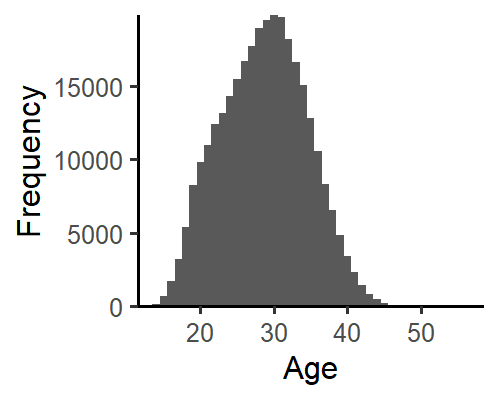
\includegraphics[width=\textwidth]{supp-img/dens_age.png}
    \vspace{.5cm}
    \end{subfigure}\hfill
    \begin{subfigure}{.3\textwidth}
        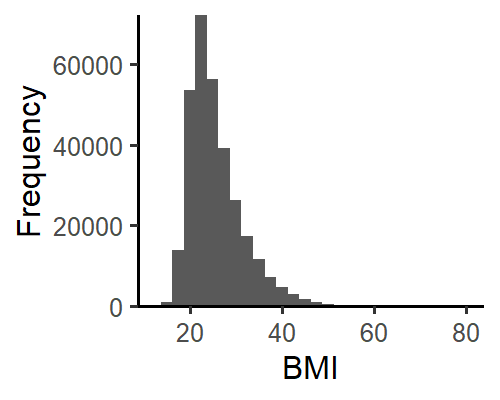
\includegraphics[width=\textwidth]{supp-img/dens_bmi.png}
    \vspace{.5cm}
    \end{subfigure}\hfill
    \begin{subfigure}{.3\textwidth}
        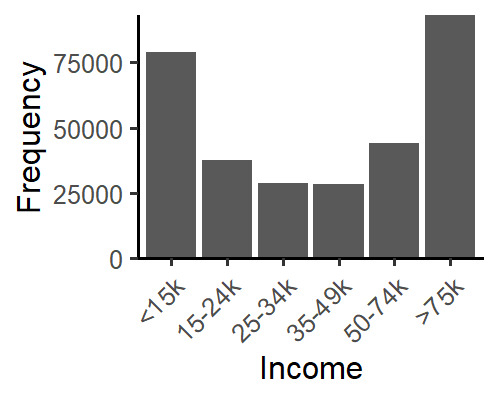
\includegraphics[width=\textwidth]{supp-img/dens_income.png}
    \vspace{.5cm}
    \end{subfigure}
    \begin{subfigure}{.3\textwidth}
        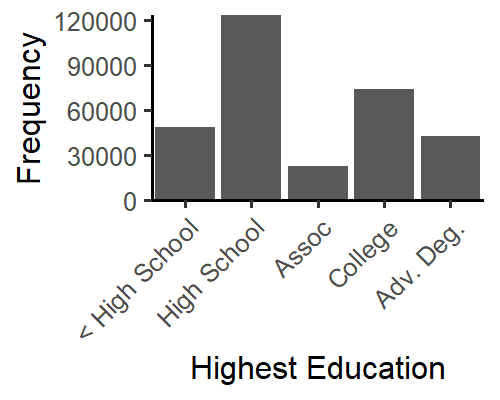
\includegraphics[width=\textwidth]{supp-img/dens_educ.png}
    \end{subfigure}\hfill
    \begin{subfigure}{.3\textwidth}
        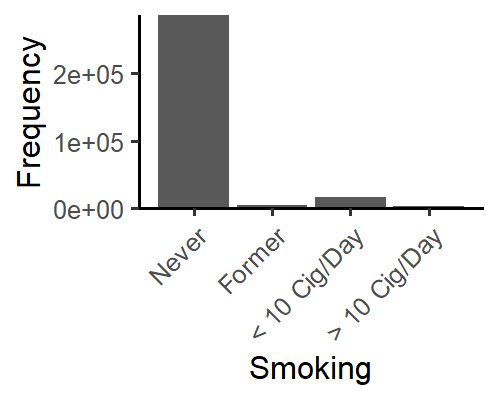
\includegraphics[width=\textwidth]{supp-img/dens_smk.png}
    \end{subfigure}\hfill
    \begin{subfigure}{.3\textwidth}
        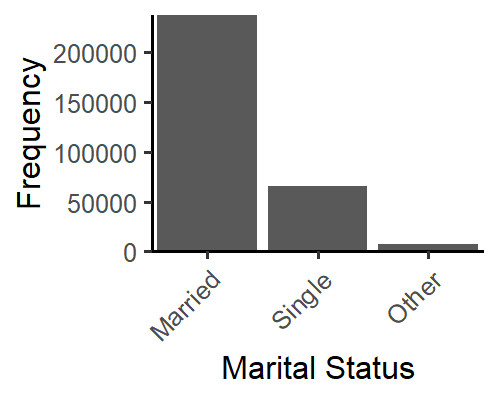
\includegraphics[width=\textwidth]{supp-img/dens_marital.png}
    \end{subfigure}
    \caption{Distribution of modifying covariates used in HDLM.}
    \label{fig:mod-dens}
\end{figure}

\begin{figure}[!ht]
    \centering
    \begin{subfigure}{.3\textwidth}
        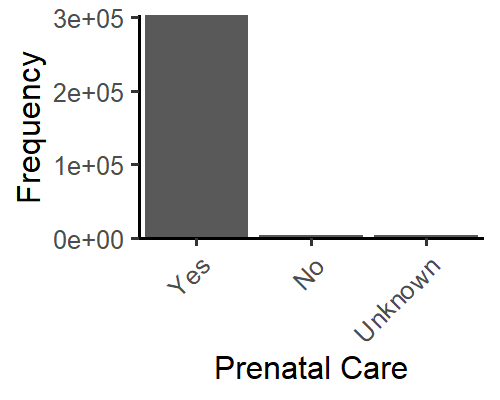
\includegraphics[width=\textwidth]{supp-img/dens_pren.png}
    \vspace{.5cm}
    \end{subfigure}\hfill
    \begin{subfigure}{.3\textwidth}
        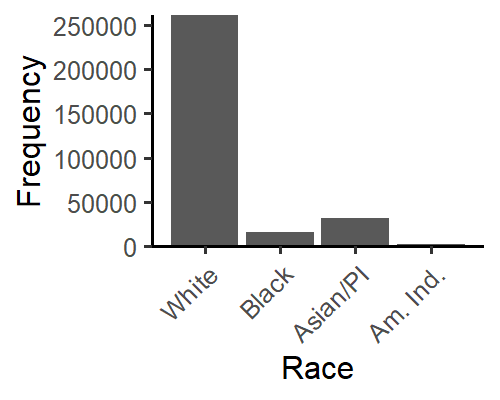
\includegraphics[width=\textwidth]{supp-img/dens_race.png}
    \vspace{.5cm}
    \end{subfigure}\hfill
    \begin{subfigure}{.3\textwidth}
        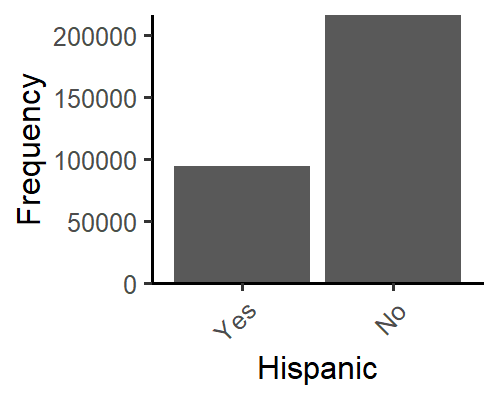
\includegraphics[width=\textwidth]{supp-img/dens_hisp.png}
    \vspace{.5cm}
    \end{subfigure}
    \begin{subfigure}{.3\textwidth}
        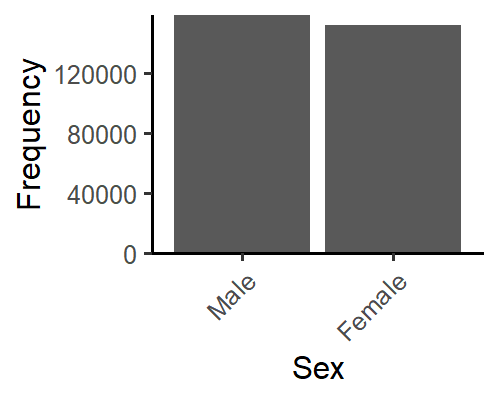
\includegraphics[width=\textwidth]{supp-img/dens_sex.png}
    \end{subfigure}
    \caption{Distribution of modifying covariates used in HDLM (continued).}
    \label{fig:mod-dens2}
\end{figure}




\subsection{MCMC Convergence Diagnostics}
To assess convergence we compared multiple MCMC chains for similar results. In addition, we estimated the distributed lag effects from two chains across iterations for four groups (Non-Hispanic and Hispanic with BMI above or below 22.8) and calculated the convergence diagnostic $\hat{R}$ for each time point \citep{Gelman1992InferenceSequences}. The largest $\hat{R}$ across all considered group/time distributed lag effects was 1.11 while the average $\hat{R}$ overall was 1.028, indicating adequate convergence. Figure \ref{fig:trace} shows trace plots for a sample of distributed lag effects considered for convergence. The trace plots also convey the model has reached convergence within the number of MCMC iterations used for our analysis.

\begin{figure}[!ht]
    \centering
    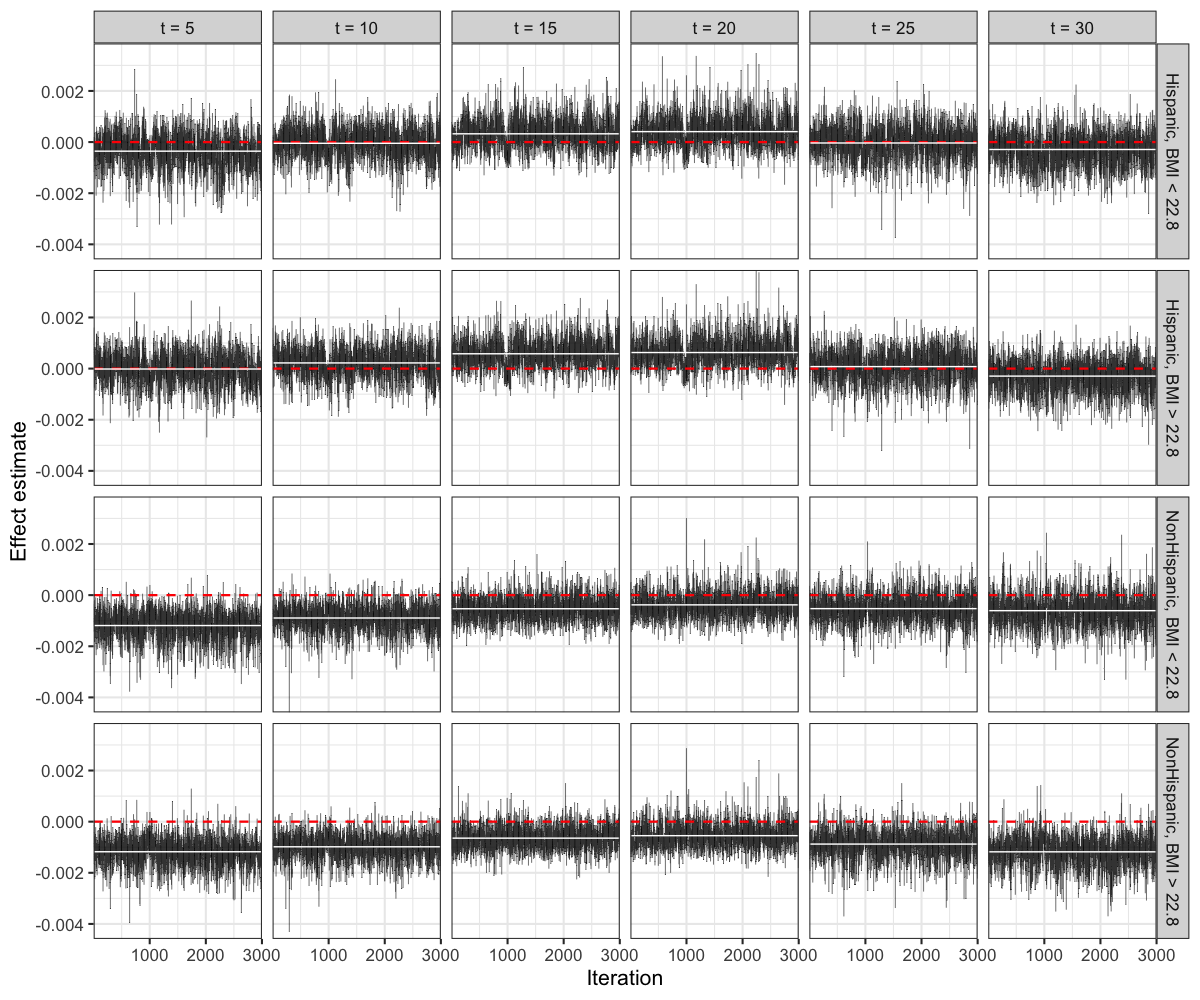
\includegraphics[width=\textwidth]{supp-img/dlm_traceplots.png}
    \caption{Trace plots of selected group (row facets) DLM effects (y-axis) at a range of lag times (column facets). The dotted red line shows zero effect and the solid white line indicates the posterior mean of the respective group/time distributed lag effect.}
    \label{fig:trace}
\end{figure}




\subsection{Effect modification}
Table \ref{tab:data_mod} compares modifier posterior inclusion probabilities among shared, nested, and Gaussian process HDLMs. We note that age, BMI, education, and Hispanic designation modifiers have the highest posterior inclusion probabilities across all three models.

\begin{table}[!ht]
\footnotesize
    \centering
    \caption{Modifying covariate posterior inclusion probabilities for three HDLM methods.}
    \label{tab:data_mod}
    \begin{tabular}{lccc}
        \toprule[2pt]
        Modifier & Shared Tree & Nested Tree & Gaussian Process\\
        \hline
        Age at conception &  0.93 & 0.90 & 0.83\\
        Body mass index & 0.95 & 0.96 & 0.96\\
        Income range &  0.74 & 0.71 & 0.72\\
        Highest education & 0.90 & 0.88 & 0.86\\
        Smoking habits &  0.78 & 0.76 & 0.81\\
        Marital status &  0.50 & 0.46 & 0.45\\
        Prenatal care &  0.48 & 0.60 & 0.54\\
        Race & 0.61 & 0.48 & 0.54\\
        Hispanic & 0.95 & 0.98 & 0.90\\
        Sex of child & 0.64 & 0.43 & 0.53\\
        \bottomrule
    \end{tabular}
\end{table}


Figure \ref{fig:pip-cont} describes the posterior distribution of splitting rules for age and BMI, with modes at 27 and 22.8, respectively. Figure \ref{fig:pip-int} illustrates the PIP of interactions between modifiers. In simulation, the average PIP for non-active modifier interactions was 0.11. We found the highest interaction PIPs to be education--BMI (0.65), education--age (0.64), and BMI--Hispanic (0.57).

\begin{figure}
    \centering
    \begin{subfigure}{.46\textwidth}
        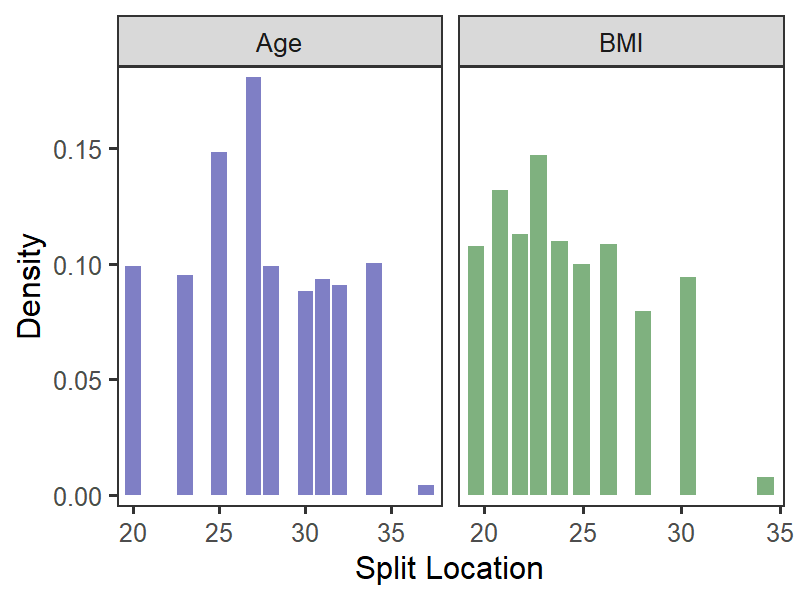
\includegraphics[width=.95\textwidth]{supp-img/bwgaz_cont_split.png}
        \caption{}
        \label{fig:pip-cont}
    \end{subfigure}
    \begin{subfigure}{.45\textwidth}
        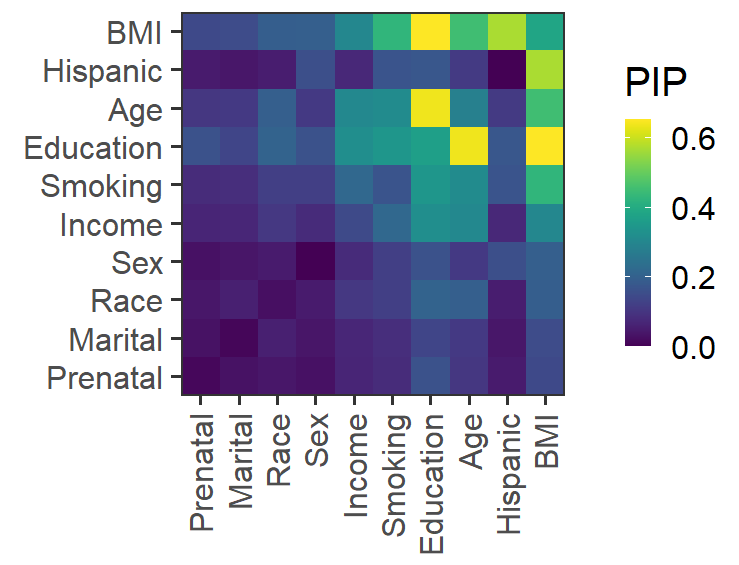
\includegraphics[width=.95\textwidth]{supp-img/bwgaz_pip_int.png}
        \caption{}
        \label{fig:pip-int}
    \end{subfigure}
    \caption{Panel (a) shows the posterior distribution of splitting rules for two continuous modifiers: maternal age and BMI. Panel (b) shows posterior inclusion probability (PIP) of modifier interactions.}
    \label{fig:pip}
\end{figure}

\subsection{Additional Figures}
Figure \ref{fig:mspe} shows the MSPE results from 10-fold cross-validation of the three HDLMs relative to a treed DLM without effect modification. On average, the MSPE of the shared tree HDLM was smallest (0.99975) followed by nested tree HDLM (0.99979) and Gaussian process HDLM (0.99982). The signal of the exposure effect is very small relative to the signal from the fixed effects and residual error, leading to very small differences between the MSPE for these methods.
\begin{figure}[!ht]
    \centering
    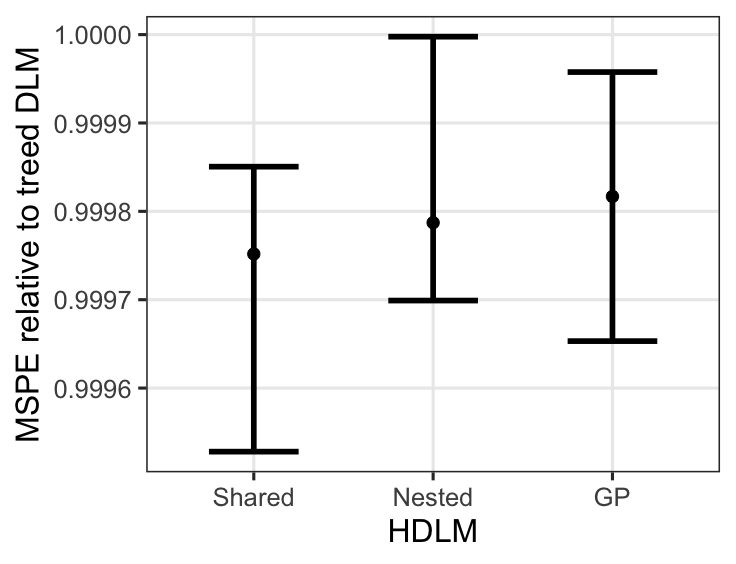
\includegraphics[width=.4\textwidth]{supp-img/mspe.png}
    \caption{MSPE of HDLMs relative to treed DLM without modification. Error bars show MSPE interquartile range and dots indicate the average MSPE from 10-fold cross-validation.}
    \label{fig:mspe}
\end{figure}

Figure \ref{fig:est_tdlm} shows the results from the treed DLM without effect modification.

\begin{figure}[!ht]
    \centering
    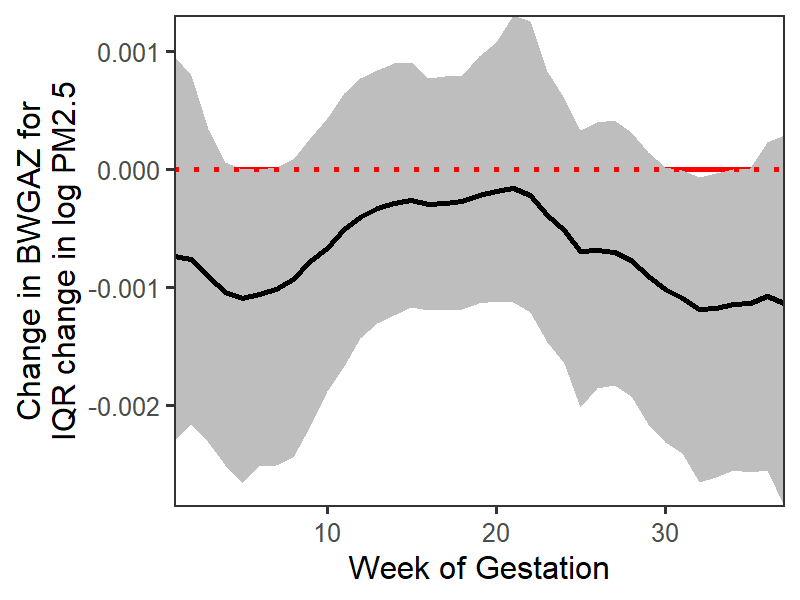
\includegraphics[height=5cm]{supp-img/bwgaz_tdlm.png}
    \caption{Estimated distributed lag functions due to an IQR increase in PM$_{2.5}$ using the treed DLM with no effect modification. The solid line indicates the posterior mean while the gray area represents a 95\% credible interval. Weeks where the credible interval does not contain zero represent critical windows.}
    \label{fig:est_tdlm}
\end{figure}

Figure \ref{fig:hisp-nonhisp} shows subgroup-specific DLMs for Hispanic vs non-Hispanic.
\begin{figure}[!ht]
    \centering
    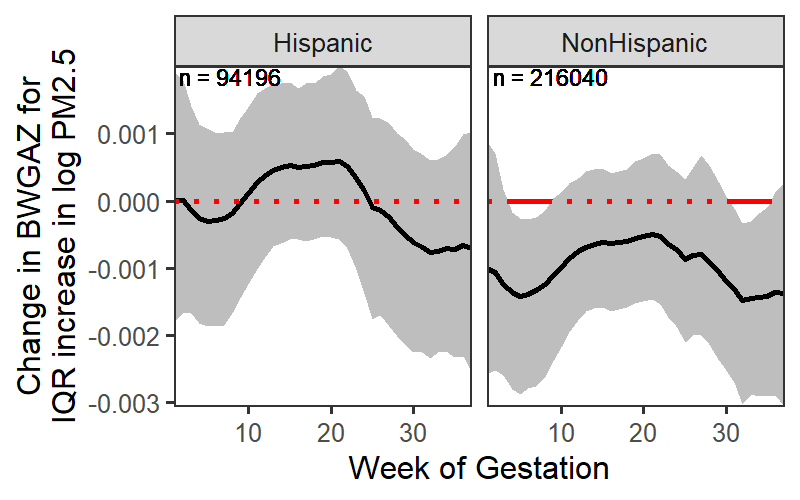
\includegraphics[width=.5\textwidth]{supp-img/bwgaz_hisp_nonhisp.png}
    \caption{Hispanic and non-Hispanic subgroup-specific DLMs.}
    \label{fig:hisp-nonhisp}
\end{figure}

Figures \ref{fig:hisp-educ-age} and \ref{fig:hisp-educ-bmi} show the Hispanic subgroup broken down by education and age, as well as education and BMI, respectively.
\begin{figure}[!ht]
    \centering
    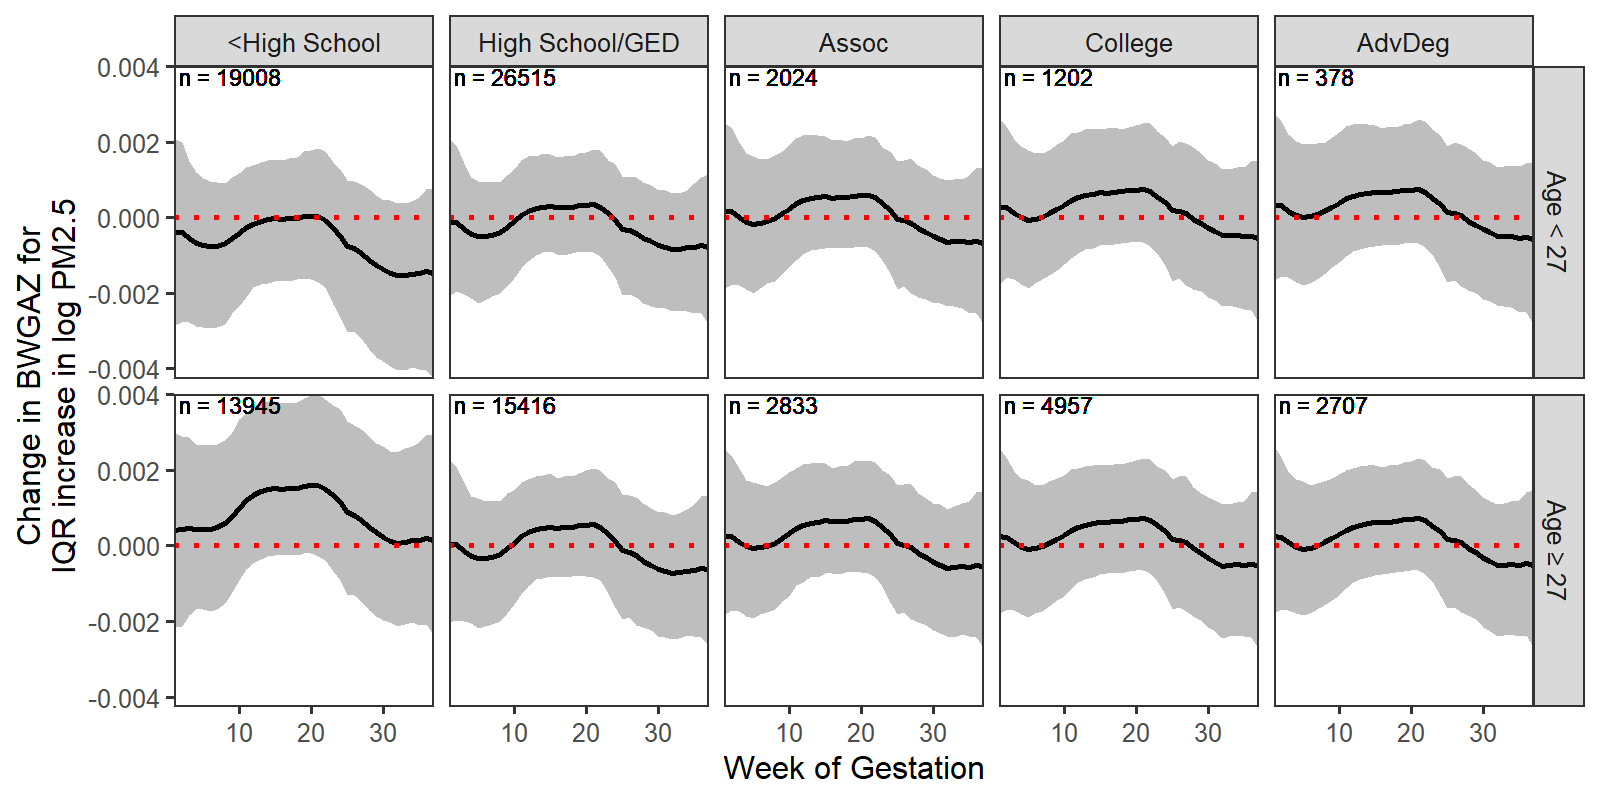
\includegraphics[width=.9\textwidth]{supp-img/hisp_educ_age.png} 
    \caption{Hispanic subgroup broken out by education and age.}
    \label{fig:hisp-educ-age}
\end{figure}
\begin{figure}[!ht]
    \centering
    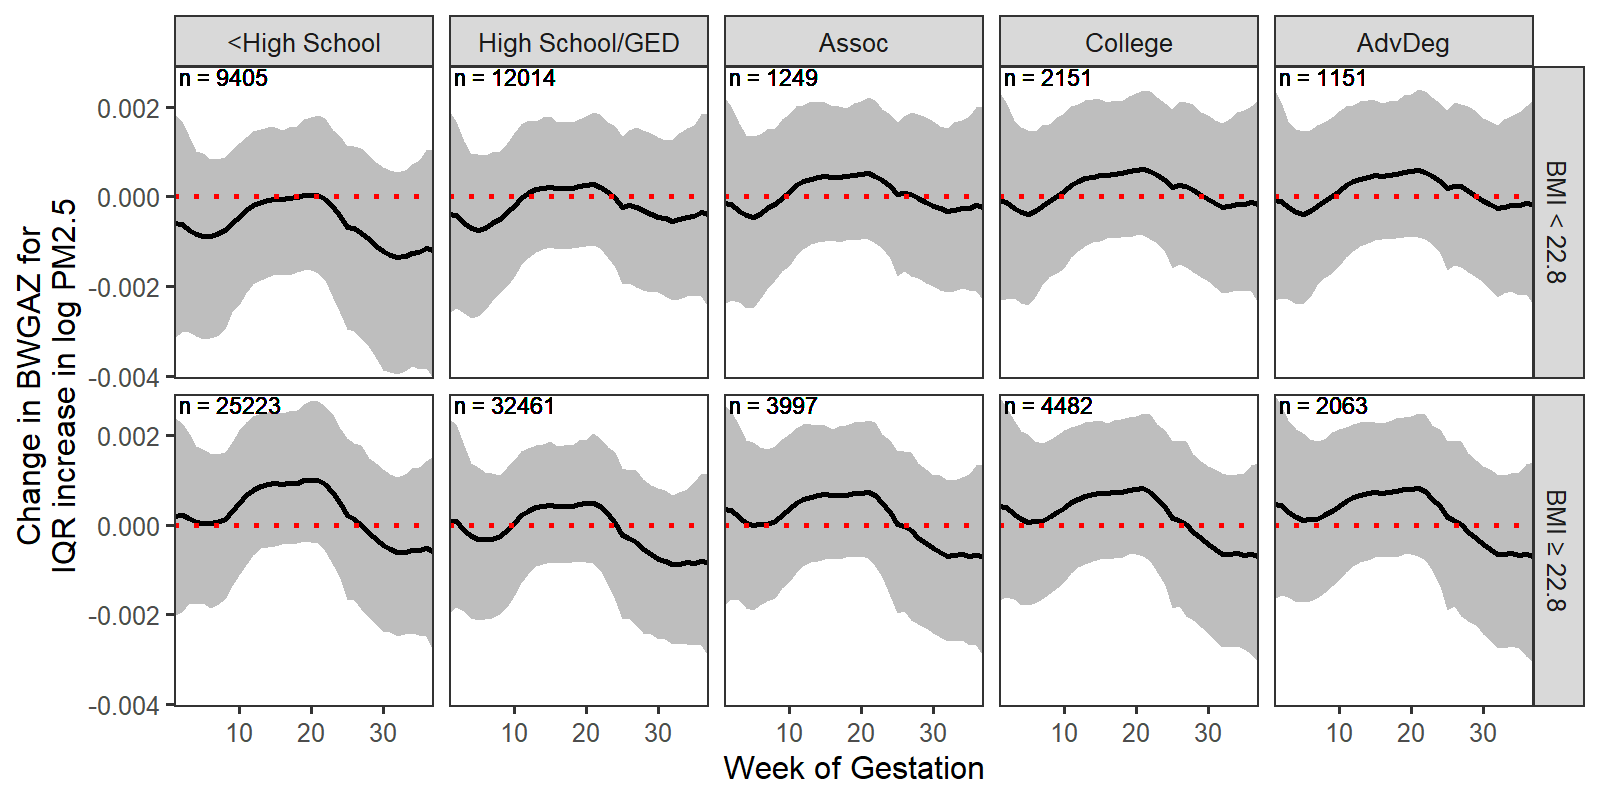
\includegraphics[width=.9\textwidth]{supp-img/hisp_educ_bmi.png}
    \caption{Hispanic subgroup broken out by education and BMI.}
    \label{fig:hisp-educ-bmi}
\end{figure}

Figures \ref{fig:nonhisp-educ-age} and \ref{fig:nonhisp-educ-bmi} show the non-Hispanic subgroup broken down by education and age, as well as education and BMI, respectively.
\begin{figure}[!ht]
    \centering
    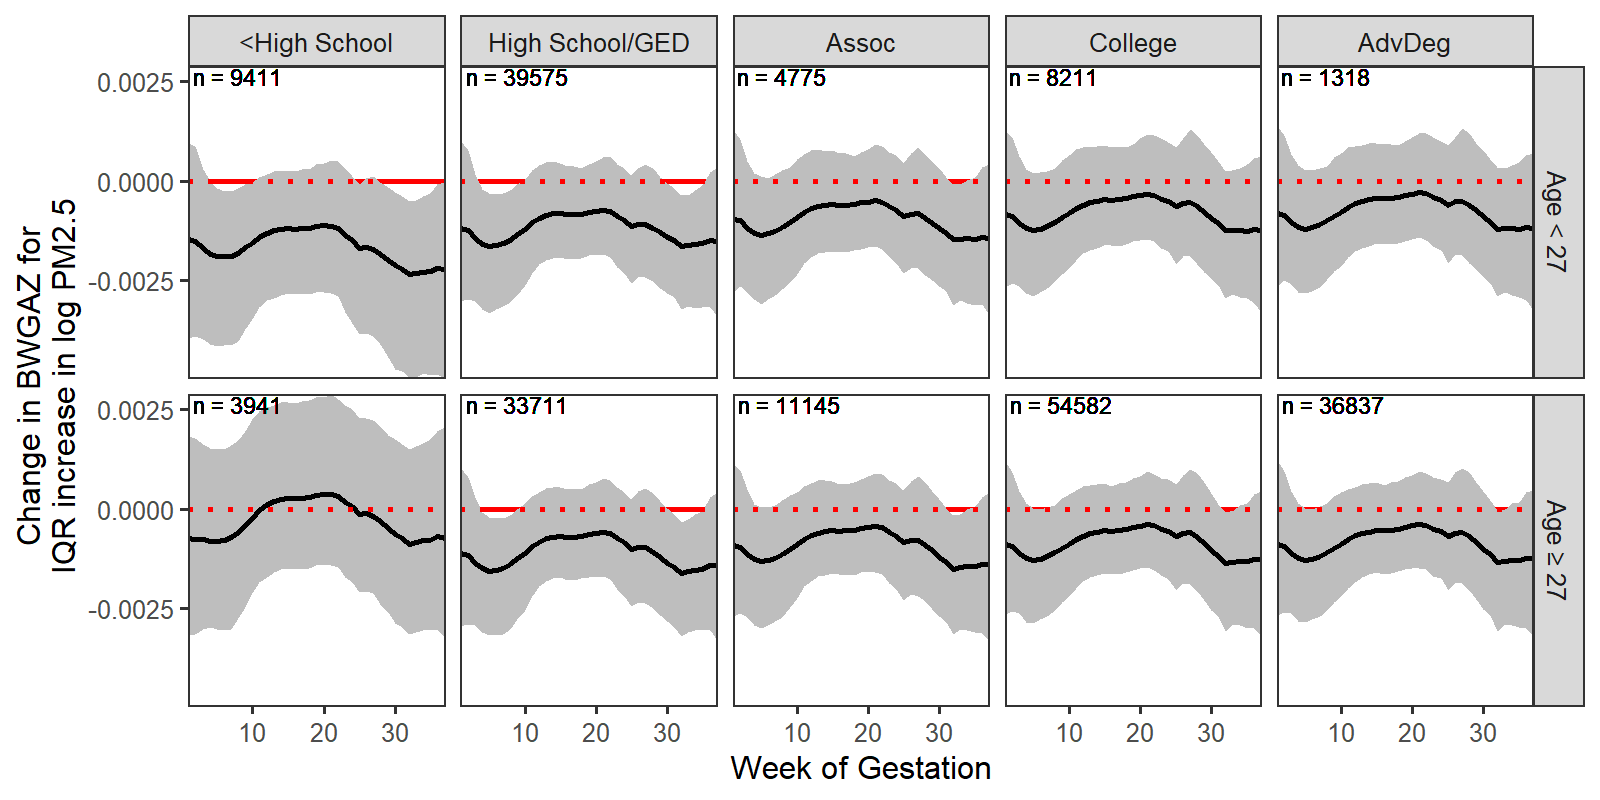
\includegraphics[width=.9\textwidth]{supp-img/nonhisp_educ_age.png}
    \caption{Non-Hispanic subgroup broken out by education and age.}
    \label{fig:nonhisp-educ-age}
\end{figure}
\begin{figure}[!ht]
    \centering
    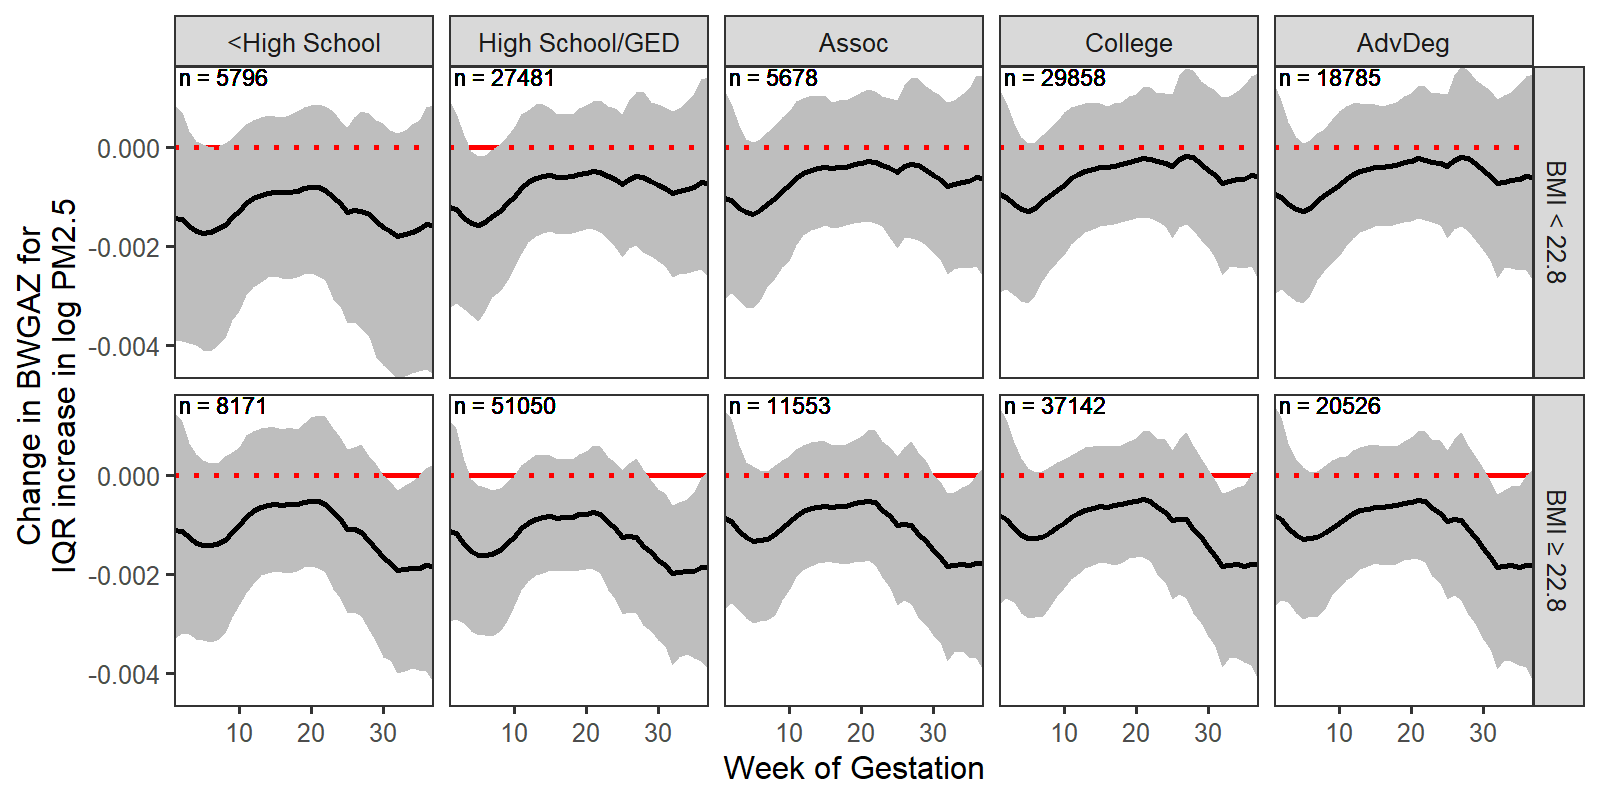
\includegraphics[width=.9\textwidth]{supp-img/nonhisp_educ_bmi.png}
    \caption{Non-Hispanic subgroup broken out by education and BMI.}
    \label{fig:nonhisp-educ-bmi}
\end{figure}

The next largest modifier PIP was Smoking and the next largest modifier interaction PIP was between smoking and BMI. Figures \ref{fig:hisp-smk-bmi} and \ref{fig:nonhisp-smk-bmi} show subgroup-specific DLMs for Hispanic and non-Hispanic subgroups broken down by smoking (never vs. former or current) and BMI.
\begin{figure}[!ht]
    \centering
    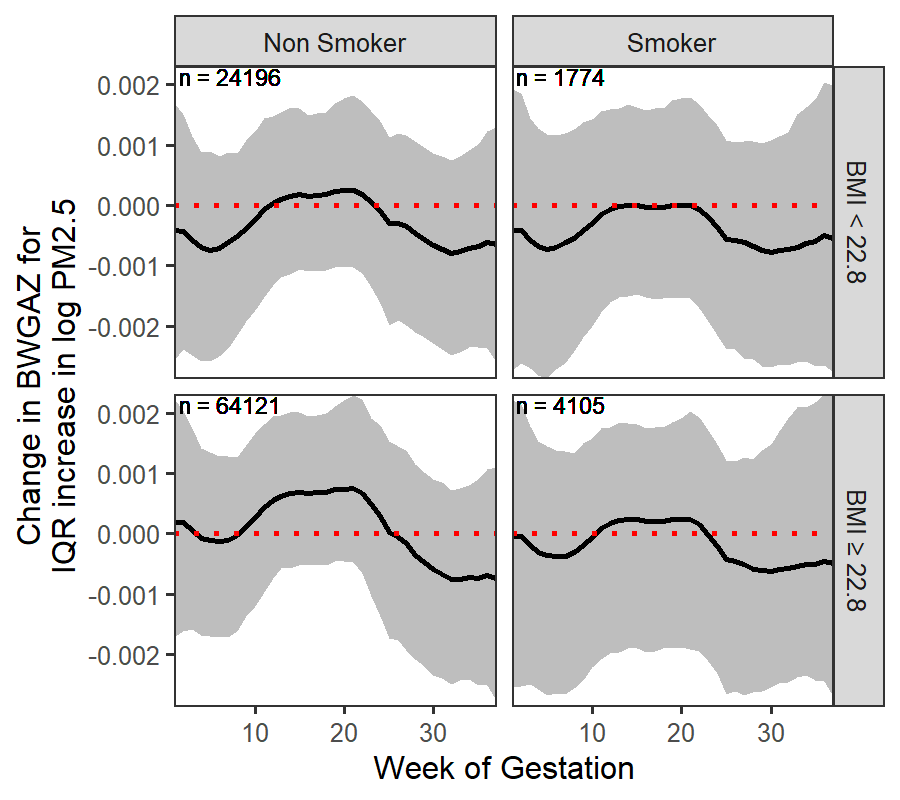
\includegraphics[width=.5\textwidth]{supp-img/hisp_smk_bmi.png}
    \caption{Hispanic subgroup broken out by smoking (never vs former or current) and BMI.}
    \label{fig:hisp-smk-bmi}
\end{figure}
\begin{figure}[!ht]
    \centering
    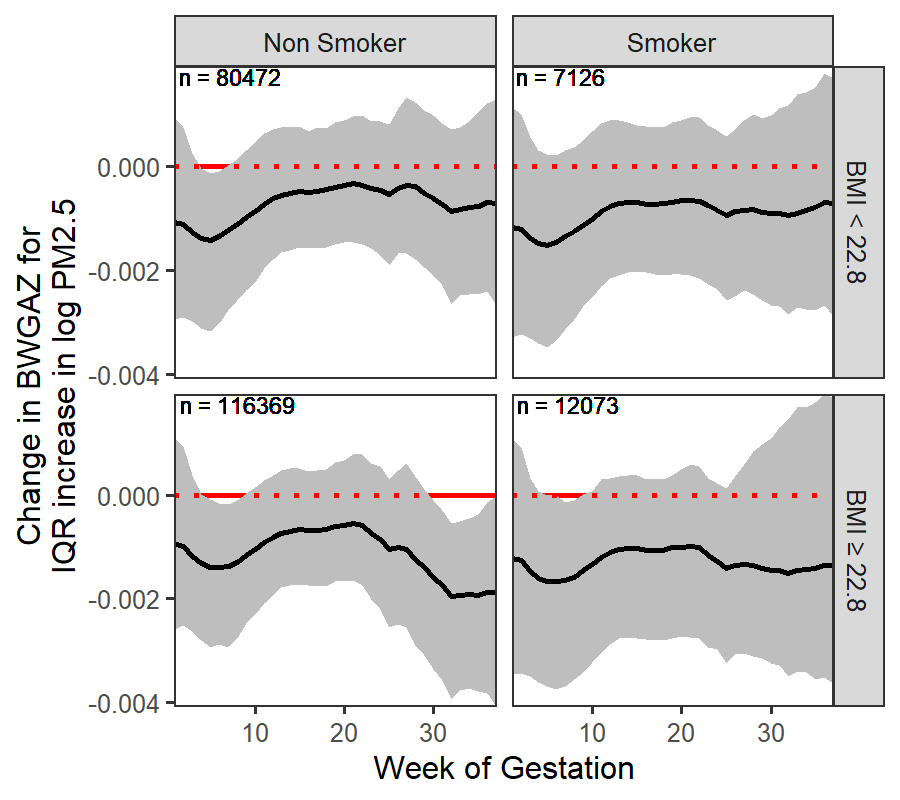
\includegraphics[width=.5\textwidth]{supp-img/nonhisp_smk_bmi.png}
    \caption{Non-Hispanic subgroup broken out by smoking (never vs former or current) and BMI.}
    \label{fig:nonhisp-smk-bmi}
\end{figure}
\clearpage


\subsection{Nested Tree HDLM}
We replicate the subgroup-specific analyses of the paper using the nested tree HDLM. Figure \ref{fig:nested-hisp-bmi} shows subgroup specific DLMs broken down by Hispanic and BMI modifiers. Figure \ref{fig:nested-hisp-educ} shows subgroup specific DLMs broken down by Hispanic and education modifiers. 


\begin{figure}[!ht]
    \centering
    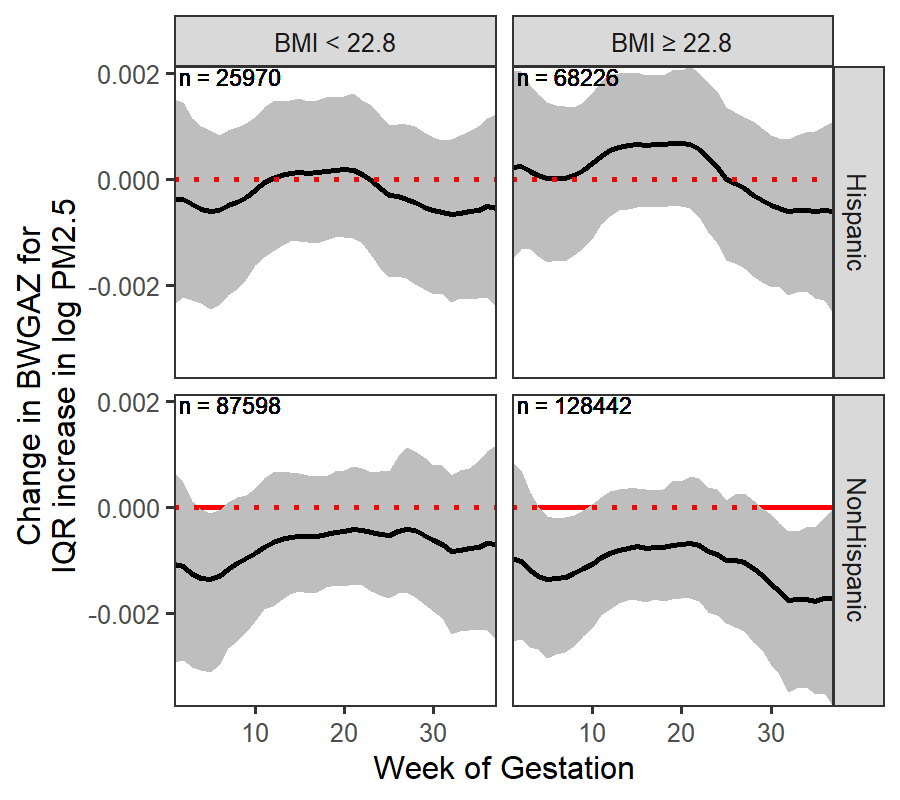
\includegraphics[width=.5\textwidth]{supp-img/nested_hisp_bmi.png}
    \caption{Subgroup-specific DLMs broken down by Hispanic and BMI, using the nested tree HDLM.}
    \label{fig:nested-hisp-bmi}
\end{figure}
\begin{figure}[!ht]
    \centering
    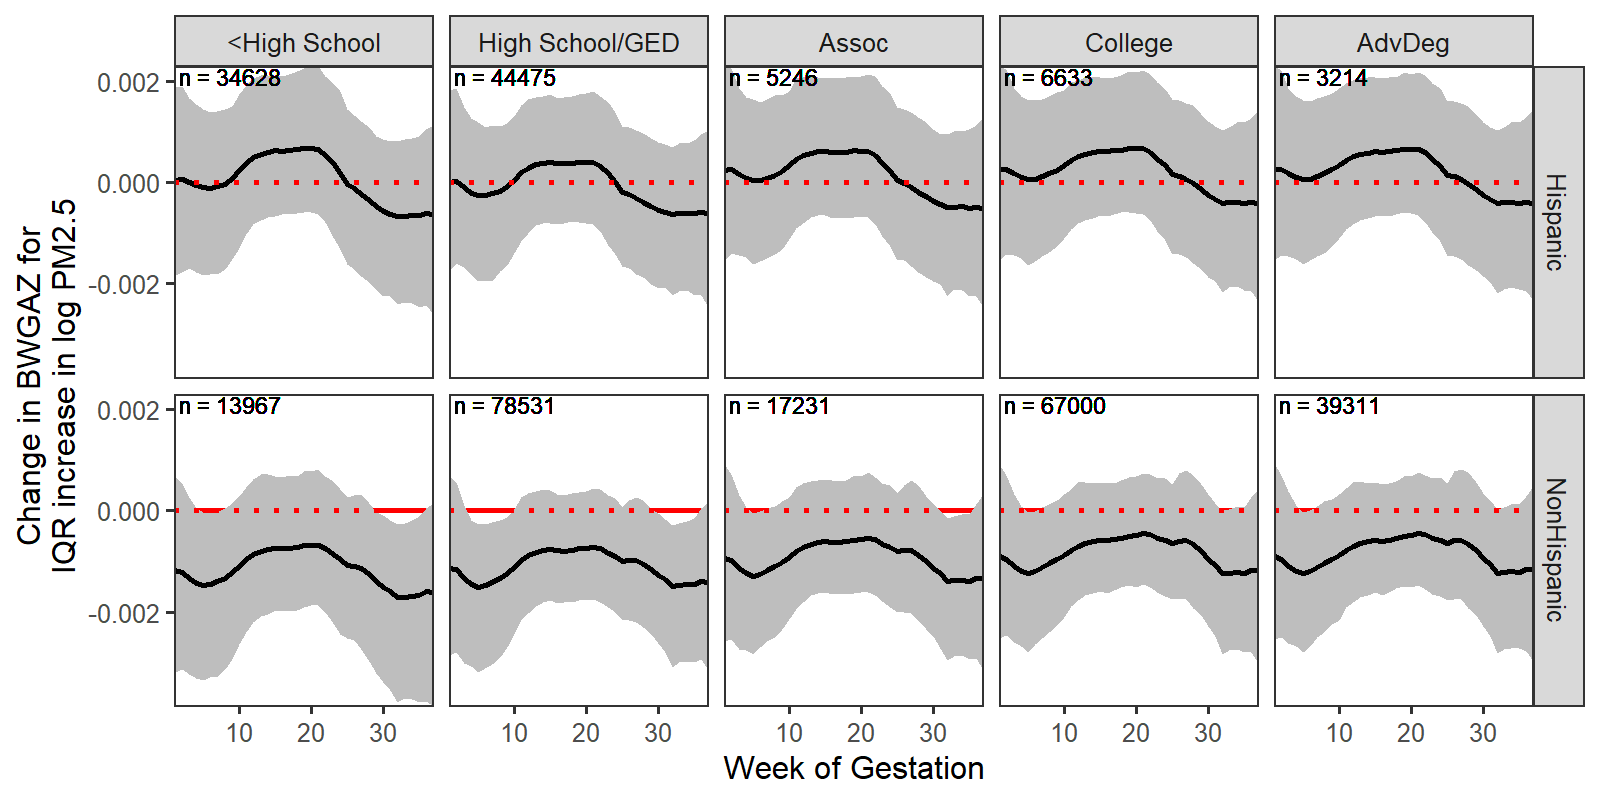
\includegraphics[width=.9\textwidth]{supp-img/nested_hisp_edu.png}
    \caption{Subgroup-specific DLMs broken down by Hispanic and education, using the nested tree HDLM.}
    \label{fig:nested-hisp-educ}
\end{figure}

\clearpage

\subsection{Gaussian process HDLM}
We replicate the subgroup-specific analyses of the paper using the Gaussian process HDLM. Figure \ref{fig:gp-hisp-bmi} shows subgroup specific DLMs broken down by Hispanic and BMI modifiers. Figure \ref{fig:gp-hisp-educ} shows subgroup specific DLMs broken down by Hispanic and education modifiers. We note the increased variance of the distributed lag effect estimates as well as decreased smoothness in the DLM, which does not allow for critical window identification.

\begin{figure}[!ht]
	\centering
    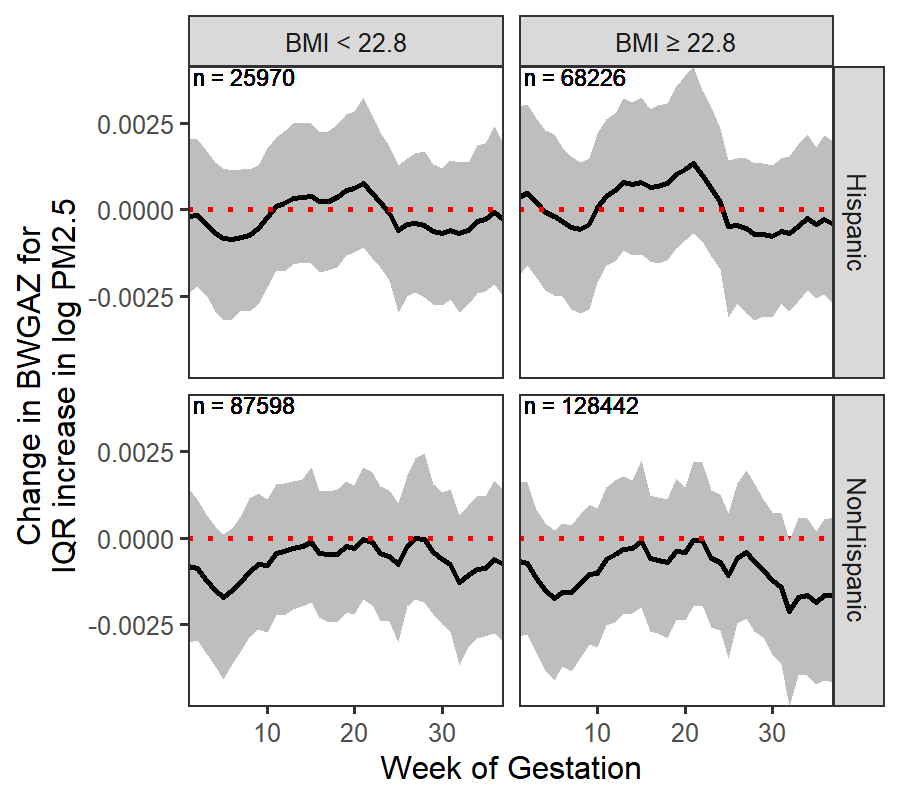
\includegraphics[width=.5\textwidth]{supp-img/gp_hisp_bmi.png}
    \caption{Subgroup-specific DLMs broken down by Hispanic and BMI, using the Gaussian process HDLM.}
    \label{fig:gp-hisp-bmi}
\end{figure}
\begin{figure}[!ht]
	\centering
    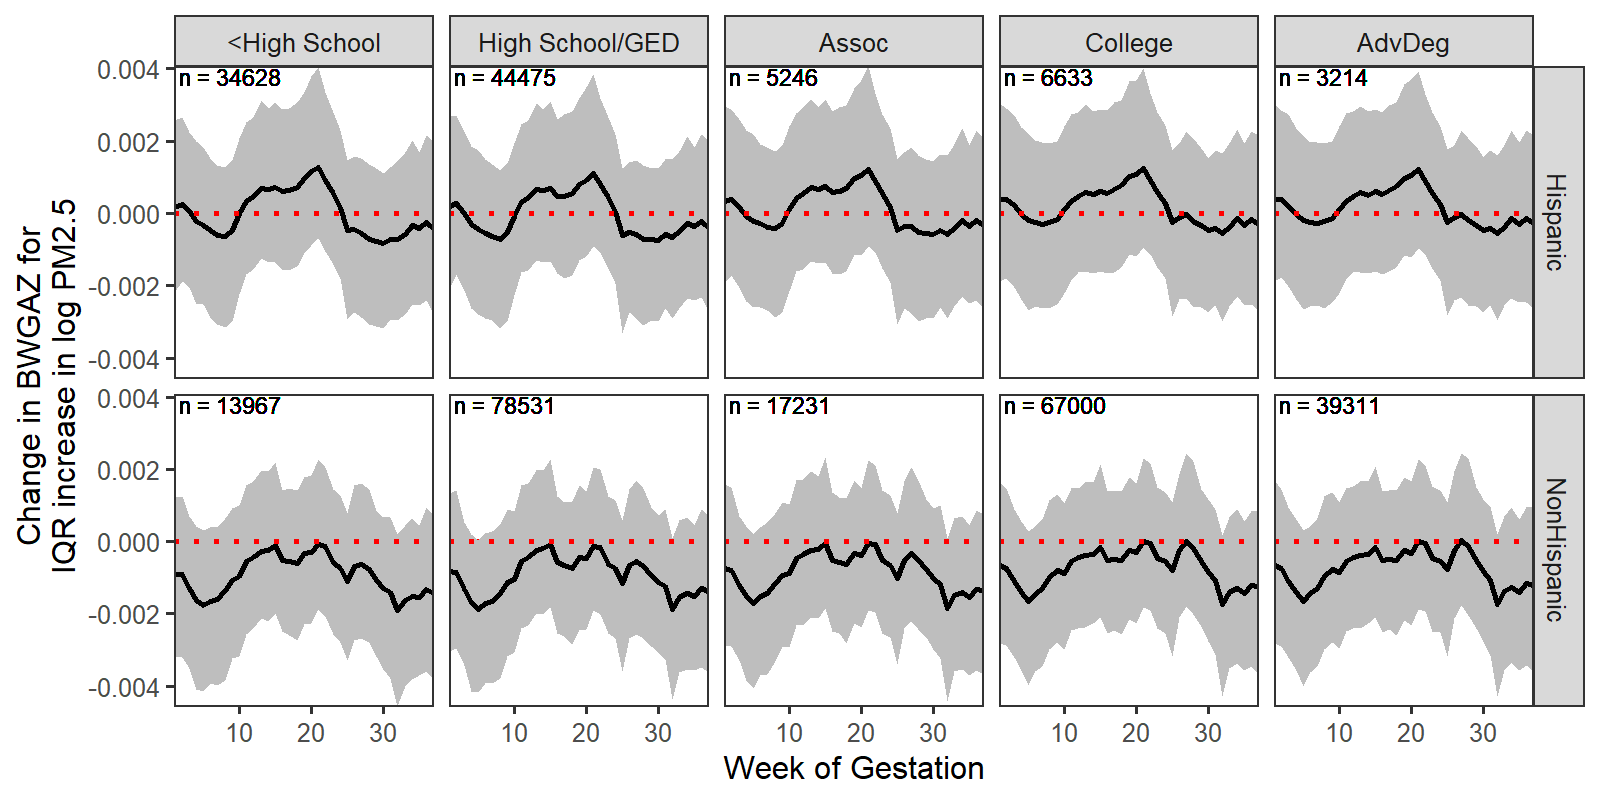
\includegraphics[width=.9\textwidth]{supp-img/gp_hisp_educ.png}
    \caption{Subgroup-specific DLMs broken down by Hispanic and education, using the Gaussian process HDLM.}
    \label{fig:gp-hisp-educ}
\end{figure}
\clearpage
%======================================
\bibliography{references}
%======================================


\end{document}

